\part*{Differential calculus}

\section*{Foundations of calculus: limits and continuity}

\subsection*{What is calculus about?}

Calculus is about \textit{measuring change} by thinking about the infinitely small. All of calculus relies on intuition about ``infinitely small numbers'', or \textit{infinitesimals}.

In \textit{differential calculus}, the concept of infinitesimals is invoked in order to measure the speed at which change occurs. If we want to measure the speed at which the output of a function $f$ is changing in response to a changing input, we can consider the rate of change of $f$ at the input $x$ to be the slope of the line that the curvy $f$ vs. $x$ graph ``becomes'' as we ``zoom in infinitely close'' to the point $(x, f(x))$.

In \textit{integral calculus}, we use infinitesimals to compute how much total change is caused by a given rate of change. If we want to determine how much total change has been caused by a rate of change that itself changes over time, we can think of the rate of change as being the aggregation of many rates of change that \textit{don't} change over time, where each of these rates occurs over an ``infinitely small'' window of input values, and then add up all of the little changes that result.

\subsection*{Limits}

The concept of ``infinitely small numbers'' is most often\footnote{There is another approach to formalizing the concept of ``infinitely small numbers'' called \textit{nonstandard analysis}. This approach is in some ways more intuitive because it literally does give a definition for ``infinitely small number''. On the other hand, nonstandard analysis requires that one drop the assumption that ``not false'' is equivalent to ``true''. Some may view this as a disadvantage. Nonstandard analysis also obscures the presence of ``error terms'' (terms that disappear in a limit taken to zero or infinity) that the limit approach makes obvious.} formalized with the concept of \textit{limits}. 

If, as inputs to a function $f$ that are \textit{greater} than a particular input $p$ get closer and closer to $p$, the outputs of $f$ get closer and closer to a number $L$, then we say ``the limit of $f$ as $x$ approaches $p$ from the right is $L$'', and write

\begin{align*}
    \lim_{x \rightarrow p^+} f(x) = L.
\end{align*}

The $+$ sign on the ``$p^+$'' below the limit indicates that the limit is taken ``from the right''; i.e., that the inputs that are getting closer to $p$ are all greater than $p$.

Similarly, if, as inputs of $f$ that are \textit{less} than $p$ get closer and closer to $p$, the outputs of $f$ get closer and closer to a number $M$, then we say ``the limit of $f$ as $x$ approaches $p$ from the left is $M$'', and write

\begin{align*}
    \lim_{x \rightarrow p^-} f(x) = M.
\end{align*}

The $-$ on the ``$p^-$'' below the limit indicates that the limit here is taken ``from the left''; the inputs that are getting closer to $p$ are all less than $p$.

If the limits of $f$ at $p$ from the left and from the right are the same, then we define the so-called \textit{two-sided limit} to be equal to the left and right limits\footnote{The colon-equals sign $:=$ is used here instead of a regular equals sign $=$ to indicate that the combination of symbols on the left side is being \textit{defined} to mean whatever is written on the right side. While some authors use the regular equals sign $=$ to denote definitions, I prefer to use the colon-equals $:=$ because I think it is important to disambiguate ``equality by definition'' from ``equality resulting from mathematical reasoning''.}:

\begin{align*}
    \lim_{x \rightarrow p} f(x) 
    := \lim_{x \rightarrow p^+} f(x) 
    = \lim_{x \rightarrow p^-} f(x).
\end{align*}

The lack of a $-$ or $+ $ sign on the ``$p$'' below the limit indicates that the limit is two-sided.

With the above formalism set up, expressions involving an ``infinitely small number'' $x$ can be reasoned about by considering limits of the form $\lim_{x \rightarrow 0} f(x)$; we can think of the $x$ in such limits as being ``infinitely close to zero''.

\subsubsection*{When limits don't exist}

It is not always the case that a given limit exists. 

A two-sided limit does not exist if its associated one-sided limits are not equal. When this is the case, and we have $\lim_{x \rightarrow p^-} f(x) \neq \lim_{x \rightarrow p^+} f(x)$, we say that $f$ has a \textit{jump discontinuity} at $p$.

Additionally, both two-sided and one-sided limits of a function $f$ at a point $p$ may fail to exist for the following reasons:

\begin{itemize}
    \item It may be the case that as inputs approach $p$, outputs only grow more and more positive or more and more negative. In these cases, the limit is considered to be \textit{infinite}, and we write something like ``$\lim_{x \rightarrow p} f(x) = \infty$'' or ``$\lim_{x \rightarrow p} f(x) = -\infty$''.
    \item It may be the case that as inputs approach\footnote{Consider $f(x) = \sin(2 \pi \omega(x) x)$, where $\omega(x) = (2 \pi x^2)^{-1}$. Since $\lim_{x \rightarrow 0^+} \omega(x) = \infty$, the graph of $f$ is a sine wave whose oscillation frequency approaches infinity as $x \rightarrow 0^+$. Thus, $f(x)$ oscillates wildly as $x \rightarrow 0^+$. This implies that $f(x)$ doesn't get closer to any particular value as $x \rightarrow 0^+$, i.e., that $\lim_{x \rightarrow 0^+} f(x)$ does not exist.} $p$, the outputs oscillate and do not settle around any particular number.
\end{itemize}

\subsubsection*{Relationship between infinite and zero limits}

It's worth noting that the statement $(\lim_{x \rightarrow p} f(x) = - \infty \text{ or } \lim_{x \rightarrow p} f(x) = \infty)$ is true exactly when $\lim_{x \rightarrow p} \frac{1}{f(x)} = 0$ is true.

\subsubsection*{Properties of limits}

The following properties of limits that we present (but do not prove) are hopefully somewhat intuitive.

\vspace{.25cm}

If $\lim_{x \rightarrow p} f(x)$ exists, then

\begin{align*}
    \lim_{x \rightarrow p} (c f(x)) = c \lim_{x \rightarrow p} f(x)
\end{align*}

If $\lim_{x \rightarrow p} f(x)$ and $\lim_{x \rightarrow p} g(x)$ both exist, then

\begin{align*}
    \lim_{x \rightarrow p} (f(x) + g(x)) &= \lim_{x \rightarrow p} f(x) + \lim_{x \rightarrow p} g(x) \\
    \lim_{x \rightarrow p} (f(x) g(x)) &= \Big( \lim_{x \rightarrow p} f(x) \Big) \Big( \lim_{x \rightarrow p} g(x) \Big) \\
    \lim_{x \rightarrow p} \frac{f(x)}{g(x)} &= \frac{\lim_{x \rightarrow p} f(x)}{\lim_{x \rightarrow p} g(x)} \text{ when } \lim_{x \rightarrow p} g(x) \neq 0
\end{align*}

The properties $\lim_{x \rightarrow p} (c f(x)) = c \lim_{x \rightarrow p} f(x)$ and $\lim_{x \rightarrow p} (f(x) + g(x)) = \lim_{x \rightarrow p} f(x) + \lim_{x \rightarrow p} g(x)$ are collectively referred to as \textit{the linearity of the limit operator}\footnote{The limit operator $\lim_{x \rightarrow p}$ can be considered to be a function that sends functions to real numbers. In general, if $\Phi$ is a function that accepts other functions as input, then $\Phi$ is said to be \textit{linear} if, for all functions $f, g$ and all real numbers $c$, we (1) have $\Phi(f + g) = \Phi(f) + \Phi(g)$ and (2) have $\Phi(cf) = c\Phi(f)$. The function $\lim_{x \rightarrow p}$ is linear in this sense.

It may seem a bit strange that such functions are called ``linear functions''- after all, what do they have to do with lines? For the answer to this question, you will want to take a course in \textit{linear algebra}. The short answer is: inputs to linear functions are themselves ``linear elements'', and linear functions by definition ``preserve the decomposition'' of linear elements; linear functions are called what they are because they play nicely with linear elements.}. The last two properties are called the \textit{product rule for limits} and the \textit{quotient rules for limits}, respectively.
    
\subsubsection*{Limits at infinity}

Another useful notion brought to us by the intuition of limits\footnote{I'm hinting here that the technical mathematical definition of a limit at infinity ($\lim_{x \rightarrow \infty} f(x)$, $\lim_{x \rightarrow -\infty} f(x)$) is different than the technical mathematical definition of a limit at a point ($\lim_{x \rightarrow p} f(x)$). This is due to the fact that we have to make some formal interpretation of what we mean by $x \rightarrow \infty$ and $x \rightarrow -\infty$; this interpretation involves $|x|$ getting larger and larger, which is different than the ``getting closer and closer'' involved in the definition of limit at a point.} is that of a function's ``limits at infinity'', or ``end behavior''. The idea is that, for a function $f$, we write $\lim_{x \rightarrow \infty} f(x) = L$ if, as $x$ gets larger and larger, $f(x)$ gets closer and closer to a number $L$. Similarly, we write $\lim_{x \rightarrow -\infty} f(x) = M$ if, as $x$ gets lesser and lesser and veers off to negative infinity, $f(x)$ gets closer and closer to a number $M$. 

Geometrically, a function's limits at infinity are the horizontal lines that its graph approaches but never touches, i.e., the function's limits at infinity correspond to \textit{horizontal asymptotes}.

Using the definitions of limits at infinity presented above, it's possible to prove that

\begin{align*}
    \lim_{x \rightarrow \infty} \frac{1}{x} = 0 \text{ and } \lim_{x \rightarrow -\infty} \frac{1}{x} = 0. 
\end{align*}

Hopefully this is intuitive enough: make $x$ really really big, and $\frac{1}{x}$ becomes really really small.

Note that the limit product rule implies

\begin{align*}
    \lim_{x \rightarrow \infty} x^{-n} = 0 &\text{ and } \lim_{x \rightarrow -\infty} x^{-n} = 0 \text{ for all integers $n > 0$}.
\end{align*}

[Applying the squeeze theorem], we obtain

\begin{align*}
    \lim_{x \rightarrow \infty} x^{-c} = 0 &\text{ and } \lim_{x \rightarrow -\infty} x^{-c} = 0 \text{ for all $c > 0$}.
\end{align*}

\subsubsection*{Limits at infinity of a rational function}

These new facts provide us a way to take the limits at infinity of a ``rational function'', which is a function defined by $x \mapsto \frac{P(x)}{Q(x)}$, where $P(x) = p_0 + p_1 x + p_2 x^2 + ... + p_n x^n$ and $Q(x) = q_0 + q_1 x + q_2 x^2 + ... + q_m x^m$ are degree $n$ and $m$ polynomials for some $n$ and $m$, respectively. In your precalculus class, you may have had to memorize rules about how the degrees of $P$ and $Q$ determine these limits. But no memorization of silly rules is necessary: when you want to determine end behavior, take limits and see what happens!

To illustrate the point, let's now examine the end behavior of $x \mapsto \frac{P(x)}{Q(x)}$ at positive infinity:

\begin{align*}
    \lim_{x \rightarrow \infty} \frac{P(x)}{Q(x)} 
    = \lim_{x \rightarrow \infty} \frac{p_0 + p_1 x + p_2 x^2 + ... + p_n x^n}{q_0 + q_1 x + q_2 x^2 + ... + q_m x^m} 
    = \lim_{x \rightarrow \infty} \frac{\sum_{i = 1}^n p_i x^i}{\sum_{j = 1}^m q_j x^j}.
\end{align*}

We now consider three cases. It is either the case that $n > m$, $n = m$, or $n < m$. We can actually ignore the case $n > m$, since we can obtain the result for this case by following an argument that is similar to the one used for the case $n < m$. So, we can assume that either $n < m$ or $n = m$, i.e. we can assume $n \leq m$.

At this point, we rewrite the inside of the limit:

\begin{align*}
    \lim_{x \rightarrow \infty} \frac{\sum_{i = 1}^n p_i x^i}{\sum_{j = 1}^m q_j x^j} 
    = \lim_{x \rightarrow \infty} \Big( \frac{\sum_{i = 1}^n p_i x^i}{\sum_{j = 1}^m q_j x^j} \cdot \frac{x^{-n}}{x^{-n}} \Big)
    = \lim_{x \rightarrow \infty} \Big( \frac{\sum_{i = 1}^n p_i x^{i - n}}{\sum_{j = 1}^m q_j x^{j - n}} \Big).
\end{align*}

Now, we will \textit{assume} that it is valid to apply the limit quotient rule and the linearity of the limit. (We will justify this assumption retroactively). The limit becomes

\begin{align*}
    \frac{\lim_{x \rightarrow \infty} \sum_{i = 1}^n p_i x^{i - n}}{\lim_{x \rightarrow \infty} \sum_{j = 1}^m q_j x^{j - n}}
    = \frac{\sum_{i = 1}^n p_i \lim_{x \rightarrow \infty} x^{i - n}}{\sum_{j = 1}^m q_j \lim_{x \rightarrow \infty} x^{j - n}}
\end{align*}

It is only valid to apply the limit quotient rule if the limit of the denominator in the above left expression is nonzero, and it is only valid to apply the linearity of the limit if, for all $i$ and $j$, the limits in the sums of the above right expression exist or are finite. Now comes the retroactive justification- as we continue our computations, we will see that all of these conditions are satisfied\footnote{In general, if we want to use a theorem that is stated in the form ``$(\text{conditions}) \implies (\text{result})$'', it is not valid to deduce that the conditions follow as a consequence of assuming the result- this is circular reasoning. It may seem that we are doing this here, but we are actually not. It just so happens that with limit laws, the computations involved in the result are the same computations that are examined in the testing of conditions. So, we can get ahead of ourselves and compute the result while simultaneously checking the calculations to make sure that the conditions are satisfied.}.

Consider the case in which the degree of the ``top'' polynomial is lesser than the degree of the ``bottom'' polynomial, i.e., the case in which $n < m$. First, we compute the limits in the numerator. Since $i \leq n$ and $n < m$, we have $i < n \iff i - n < 0$ for all $i$. Knowing that $i - n$ is negative for all $i$ then gives us that $\lim_{x \rightarrow \infty} x^{i - n} = 0$ for all $i$, and so the numerator is $\sum_{i = 1}^m p_i \lim_{x \rightarrow \infty} x^{i - n} = \sum_{i = 1}^m (p_i \cdot 0) = 0$. As for the denominator, we know that for all $j$ we have $j < m \iff j - m < 0$, and thus $\lim_{x \rightarrow \infty} x^{j - m} = 0$ for all $j < m$. Thus, the denominator is 

\begin{align*}
    \sum_{j = 1}^m q_j \lim_{x \rightarrow \infty} x^{j - m} = \Big( \sum_{j < m} q_j \lim_{x \rightarrow \infty} x^{j - n} \Big) + q_m x^{m - m} = \sum_{j < m} (q_j \cdot 0) + q_m = q_m.
\end{align*}

Overall, we see that when $n < m$ the limit of the rational function is $\lim_{x \rightarrow \infty} \frac{P(x)}{Q(x)} = \frac{0}{q_m} = 0$. This means that when $n < m$ the graph of $\frac{P}{Q}$ has the horizontal asymptote $y = 0$. 

A similar argument as was used above shows that when $n > m$, the overall limit is $\lim_{x \rightarrow \infty} \frac{P(x)}{Q(x)} = \lim_{x \rightarrow \infty} \frac{R(x)}{S(x)}$, where $\lim_{x \rightarrow \infty} R(x) = p_n$ and $\lim_{x \rightarrow \infty} S(x) = 0$. From this it follows that $\lim_{x \rightarrow \infty} \frac{P(x)}{Q(x)} = \pm \infty$, where we determine whether $\pm$ is $+$ or $-$ by checking whether $\frac{P}{Q}$ is eventually\footnote{Graphs of polynomials may alternate between increasing and decreasing for a little while, but for every polynomial there must exist $a$ and $b$ such that the polynomial is either strictly increasing or decreasing on $(-\infty, a)$ and either strictly increasing or decreasing on $(b, \infty)$.} increasing or whether $\frac{P}{Q}$ is eventually decreasing as $x \rightarrow \infty$.

If $P$ and $Q$ have equal degrees and $n = m$, then the limit computation for the denominator is the same as the above. The limit computation for the numerator is analogous to the one for the denominator, so we end up with the overall limit $\lim_{x \rightarrow \infty} \frac{P(x)}{Q(x)} = \frac{p_n}{q_m}$. Thus, when $n = m$, the graph of $\frac{P}{Q}$ has a horizontal asymptote at $y = \frac{p_n}{q_m}$. 

This completes our analysis of all cases. Don't worry too much about the details of this derivation, and certainly do not try to memorize this derivation! If you take away anything from the above, just remember that you do \textit{not} have to memorize anything, and that you can determine the end behavior of a rational function by following a \textit{process} if need be. 

\subsection*{Continuity}

In calculus, the objects of study are what are called \textit{continuous functions}. Intuitively, continuous functions are ones whose graphs that are smooth and without gaps. We will use the mathematical tool of limits in order define what it really means for a function to be continuous:

\begin{itemize}
    \item We say that a function $f$ is \textit{continuous at a point} $p$ if $\lim_{x \rightarrow p} f(p)$ exists and $\lim_{x \rightarrow p} f(x) = f(p)$. 
    \item We say that a function $f$ is \textit{continuous everywhere}, or simply \textit{continuous}, if it is continous at every point.
\end{itemize}

It's instructive to think about how a function could fail to be continuous at a point $p$. There are two ways for a so-called \textit{discontinuity} to occur: either it is the case that $\lim_{x \rightarrow p} f(x)$ does not exist (recall, this could be due to a jump discontinuity, an infinite limit, or an oscillating limit), or it is the case that $\lim_{x \rightarrow p} f(x) \neq f(p)$. When the later occurs, $f$ is said to have a \textit{point discontinuity} at $p$. An example of a function that satisfies the later condition is

\begin{align*}
    g(x) =
    \begin{cases}
        x & x \neq 0 \\
        1 & x = 0
    \end{cases}.
\end{align*}

In this case, we have $\lim_{x \rightarrow 0} g(x) = 0 \neq 1 = g(0)$, so $g$ has a point discontinuity at $0$.

\subsubsection*{Limit of a composition}

Suppose $f$ and $g$ are functions, that $\lim_{x \rightarrow p} f(x)$ exists, and that $g$ is continuous at $\lim_{x \rightarrow p} f(x)$. In this situation, then we can compute $\lim_{x \rightarrow p} g(f(x))$ by ``bringing the limit inside the application of $g$'': 

\begin{align*}
    {\lim_{x \rightarrow p} g(f(x)) = g(\lim_{x \rightarrow p}f(x))}.
\end{align*}

\newpage

\section*{Functions and functions evaluated on inputs}

Before we dive into calculus, we need to review the difference between two concepts that are often conflated- that of a \textit{function} and that of a \textit{function evaluated on an input}. 

\begin{itemize}
    \item A \textit{function} is an association between two sets in which every item from the set of ``inputs'' is associated with at most one item from the set of ``outputs''.
    \item A \textit{function evaluated on an input} is exactly what it sounds like- it is the result of taking an item from the function's associated input set and plugging it into the function. In other words, a function evaluated on an input is an ``output'' of the function.
\end{itemize}

If $f$ is a function, and $x$ is an input, then $f(x)$ is a function evaluated on an input.

Oftentimes, people become sloppy and conflate the two notions. When someone writes, ``the function $a^2$'', they are using incorrect mathematical grammar, since $a^2$ is not a function, but instead the the result of evaluating the function $f$ defined by $f(x) = x^2$ on the input $a$. Saying ``let $f(a)$ be a function'' is also incorrect mathematical grammar, for the same reason.

\subsubsection*{Anonomyous functions}

Since it's really tedious to write things such as ``the function $f$ defined by $f(x) = x^2$'', we introduce the following new notation:

\begin{align*}
    \text{``}x \mapsto (\text{expression involving $x$}) \text{'' means ``the function sending $x$ to $(\text{expression involving $x$})$''}.
\end{align*}

Using the above notation, we can now say ``the function $x \mapsto x^2$'' instead of ``the function $f$ defined by $f(x) = x^2$''. This notation is called \textit{anonymous function notation} because it allows us to specify functions without giving them names such as $f$.

\begin{comment}
\subsection*{On ``$f$ is a function of $x$''}

In precalculus, you are likely to have heard or read statements such as ``let $f$ be a function of $x$''. This is a somewhat vague phrase. To understand what is meant by it, consider the following context. 

Suppose you are doing some calculations in which you have force $F$ ``as a function of position $x$'' and position $x$ ``as a function of time $t$''. (Don't worry if you don't know what ``force'' actually is). Formally, we have a function $F_x$ that maps position to force and a function $x_t$ that maps time to position. From these functions, we can obtain a function $F_t$ that maps time to force, defined by $F_t(t) := F_x(x_t(t))$, i.e. $F_t = F_x \circ x_t$.

Let's now consider the situation from a more general perspective. Every symbol $S$ that represents a physical quantity (such as $F$, $x$, $t$) is associated with a ``preferred symbol'' $T$. To say that $S$ has preferred symbol $T$ is to say that we prefer to think of the physical quantity represented by $S$ as depending on the physical quantity represented by $T$ rather than as depending on some other physical quantity. 

In the above example, the preferred symbol of $F$ would be $x$, since we started with the functions $F_x$ and $x_t$. $F$'s preferred symbol is \textit{not} $t$, because we did not start with the function $F_t$, and instead had to deduce it from $F_x$ and $x_t$.

[TO DO]
\end{comment}







\newpage

\section*{Introduction to derivatives}

\subsection*{The limit definition of the derivative}

Given a function $f$ that maps real numbers to real numbers, we define the \textit{derivative of $f$} to be the function $f'$ that is defined as follows:
     
\begin{align*}
     \boxed
     {
        f'(x) := \lim_{\Delta x \rightarrow 0} \frac{f(x + \Delta x) - f(x)}{\Delta x}
     }
\end{align*}

Note, we have used $:=$ instead of $=$ because we are presenting a definition rather than proving an equality. Also note that the Greek capital letter delta, $\Delta$, is used because it is a symbol associated with changes in quantities; $\Delta x$ is thought of as a small change in input. 

There is nothing special about the variable $\Delta x$ in the above definition- it is entirely possible to write the definition of the derivative without using the $\Delta$ symbol. In fact, it is common to present the definition of the derivative using the letter $h$ in the place of $\Delta x$, as follows:

\begin{align*}
    f'(x) = \lim_{h \rightarrow 0} \frac{f(x + h) - f(x)}{h}.
\end{align*}

Here is how to interpret what $f'(x)$ means. Since $\Delta x$ goes to zero in the limit, we can imagine that $\Delta x$ is an ``infinitely small number''. Thus, $f(x + \Delta x) - f(x)$ is the change in the function $f$ that results from an infinitely small change in the input $x$. Dividing this infinitesimally small change in $f$ by the infinitesimally small change in input, $\Delta x$, intuitively gives the ``instantaneous rate of change'' of $f$ at $x$ that occurs due to the changing of the input from $x$ to $x + \Delta x$. For this reason, $f'(x)$ is often called the \textit{instantaneous rate of change of $f$ at $x$}.

\subsubsection*{Secant and tangent lines}

Geometrically, the argument of the limit, $\frac{f(x + \Delta x) - f(x)}{\Delta x}$, is the slope of the so-called secant\footnote{A line is said to be \textit{secant} to a graph if it intersects the graph at two or more points.} line that passes through the points $(x, f(x))$ and $(x + \Delta x, f(x + \Delta x))$, since the ``rise over run'' ratio of this line is equal to the expression that is inside the above limit:

\begin{align*}
    \frac{f(x + \Delta x) - x}{(x + \Delta x) - x} = \frac{f(x + \Delta x) - x}{\Delta x}.
\end{align*}

When we take the limit $\Delta x \rightarrow 0$ of the slope of this secant line, the inputs $x$ and $x + \Delta x$ become infinitely close, and thus the endpoints $(x, f(x))$ and $(x + \Delta x, f(x + \Delta x))$ of the secant line become infinitely close. Intuitively, it should be clear that, if it exists, the limit approached by taking $\Delta x \rightarrow 0$ is the slope of the line that touches the graph of $f$ at the point $(x, f(x))$ and that ``aligns with the slope of the function's graph at that point''. We call this line the \textit{tangent line}\footnote{Though we were speaking of tangent lines to gain intuition about the derivative, if we are to be formal, then we actually use the derivative to define what it means for a line to be a tangent line. The \textit{tangent line} to the graph $f$ at $(x, f(x))$ is the line of slope $f'(x)$ that passes through $(x, f(x))$.} to $f$ at $(x, f(x))$.

\subsubsection*{Differentiability}

When the derivative of a function $f$ exists at an input $p$, we say that \textit{$f$ is differentiable at $p$}.

If $f$ is differentiable at all inputs $p$, we say \textit{$f$ is differentiable}.

\subsubsection*{Continuity is a requirement for differentiability}

[TO DO]

[diff => cont, but cont =/> diff]

\subsection*{Leibniz notation}
     
So far, we have decided to denote the derivative of a function $f$ with the notation $f'$. However, there is a much more intuitive way to notate derivatives. We define the following notation:

\begin{align*}
    \frac{df(g(x))}{dg(x)} := f'(g(x)) \text{ for all functions $g$}. 
\end{align*}

In particular, we have

\begin{align*}
    \frac{df(x)}{dx} = f'(x).
\end{align*}

This notation aids intuition because you can informally think of $\frac{df(x)}{dx}$ as corresponding to dividing an infinitesimal ``rise'' at $x$, $df(x)$, by the infinitesimal ``run'' at $x$, $dx$, to get $(\text{instantaneous slope at $x$)} = \frac{\text{infinitesimal rise}}{\text{infinitesimal run}} = \frac{df(x)}{dx}$. Recall that this is the idea that is formalized in the definition of the derivative as a limit.

The notations $f'(g(x))$ and $f'(x)$ are said to be \textit{prime notation}, and the notations $\frac{df(g(x))}{dg(x)}$ and $\frac{df(x)}{dx}$ are said to be \textit{Leibniz notation}.

\subsubsection*{Leibniz operator notation}
         
You can write $\frac{df(g(x))}{dg(x)}$ in ``operator'' notation with the following new definition:

\begin{align*}
    \frac{d}{dg(x)}f(x) := \frac{df(g(x))}{dg(x)} = f'(g(x)).
\end{align*}

In particular, we have

\begin{align*}
    \frac{d}{dx}f(x) = f'(x).
\end{align*}

\subsubsection*{Leibniz vertical bar notation}

When we prefer to think of $f$ as changing in response to an input that is specifically associated with the symbol $x$ but want to evaluate $f'$ at a point $p$, we \textit{can} do so by using the fact $\frac{df(p)}{dp} = f'(p)$. This is not intuitive, however; the presence of $p$ in $\frac{df(p)}{dp}$ associates the letter $p$ with the input (we would rather that the letter $x$ be associated with the input). To remedy this situation, we define the following notation involving a vertical bar:

\begin{align*}
    \frac{df}{dx}\Big|_p &:= f'(p).
\end{align*}

One oddity of this notation is that the letter in the ``denominator'' of the derivative on the left side of the above is irrelevant: we have $\frac{df}{da}\Big|_p = \frac{df}{db}\Big|_p = \frac{df}{dc}\Big|_p = ... = \frac{df}{dz}\Big|_p$.

\subsubsection*{The most common abuse of Leibniz notation.}

People often write $\frac{df}{dx}$ to mean either $f'$ or $f'(x)$. 

Using $\frac{df}{dx}$ to mean $f'$ leads to more notation problems (see ``Single-variable calculus derivative notation'' in the appendix), and using $\frac{df}{dx}$ to mean $f'(x)$ is also confusing because it conflicts with the practice of using $\frac{df}{dx}$ to mean $f'$.

In this book, we will not ever use the notation $\frac{df}{dx}$ in this book; only $f'$, $f'(x)$, $\frac{df(g(x))}{dg(x)}$, $\frac{df(x)}{dx}$, $\frac{d}{dx}f(x)$, and $\frac{df}{dx}\Big|_p$.

\subsection*{More on derivative notation}

\indent \textbf{The advantage of prime notation; on functions versus functions evaluated at inputs.} 
         
In light of the above ``most common abuse of Leibniz notation'', prime notation is best for illustrating the fact that the derivative $f'$ of a function $f$ is itself a function. Leibniz notation does not address this subtlety, because, ``in the wild'', the symbol $\frac{df}{dx}$ can mean either $f'$ (which is a function) or $f'(x)$ (which is a function evaluated at an input).

\vspace{.5cm}

\textbf{Advantages of Leibniz notation.} 
         
You should use Leibniz notation, because, as mentioned before, it makes derivatives \textit{appear} to be fractions. This helps with intuition a lot.
         
One important example of this is that Leibniz notation can also help you remember the units of a derivative. For example, if the output of $f$ has units of length, and the input $x$ of $f$ has units of time, then you can reason that the tiny increments in $f$ and $x$, $df(x)$ and $dx$, must also have units of length and time, respectively. This lets you realize that $\frac{df(x)}{dx}$ has units of $\frac{\text{length}}{\text{time}}$.
         
Lastly, Leibniz notation helps you to remember the \textit{chain rule} for derivatives. The chain rule, which we will soon learn, is: ``$\frac{dg(f(x))}{dx} = \frac{dg(f(x))}{df(x)} \frac{df(x)}{dx}$''. Notice that it \textit{looks like} the $df(x)$'s on the right side cancel with each other to give the left side.
         
\section*{Differentiation formulas}

Now that we have developed some sense of the various derivative notations, we are ready to derive (i.e. prove) some facts that allow us to compute derivatives of complicated expressions by means of computing derivatives of simpler sub-expressions.

In this section- and book in general- I am not a stickler about stating the conditions that must be satisfied for a fact about derivatives to be applicable. I will make note of conditions when doing derivations, but will not restate them in final ``boxed'' formulas. Focusing on such conditions is not really relevant for an introduction to calculus, and, anyways, the conditions are usually self-evident from the formula in question. If a derivative formula involves some derivative $g'(x)$, well, then one of the conditions is probably ``$g$ is differentiable''!

\subsection*{The power rule}

The derivative formula that pretty much everyone learns first is the formula for $\frac{d}{dx} x^n$, when $n$ is an integer. We derive the formula by starting from the definition of the derivative, which tells us

\begin{align*}
    \frac{d}{dx} x^n = \lim_{h \rightarrow 0} \frac{(x + h)^n - x^n}{h}.
\end{align*}

To evaluate this limit, we need to figure out how to rewrite the product $(x + h)^n = \underbrace{(x + h) ... (x + h)}_{\text{$n$ times}}$ as a sum. The binomial theorem tells us how to do this; recall that it says

\newcommand*{\permcomb}[4][0mu]{{{}_{#3}\mkern#1#2_{#4}}}
\newcommand*{\perm}[1][-3mu]{\permcomb[#1]{P}}
\newcommand*{\comb}[1][-1mu]{\permcomb[#1]{C}}

\begin{align*}
    (x + h)^n = \comb{n}{0} x^n h^0 + \comb{n}{1} x^{n - 1} h^1 + \comb{n}{2} x^{n - 2} h^2 ... + \comb{n}{n} x^0 h^n,
\end{align*}

where $\comb{n}{k} = \frac{n!}{k!(n - k)!}$ is the number of unique $k$-element subsets of an $n$-element set. Noting that $\comb{n}{0} = 1$ and $\comb{n}{1} = n$, we have

\begin{align*}
    \lim_{h \rightarrow 0} \frac{(x + h)^n - x^n}{h} &=
    \lim_{h \rightarrow 0} \frac{x^n + nx^{n - 1}h + (\comb{n}{2} x^{n - 2} h^2 + ... + \comb{n}{n} x^0 h^n) - x^n}{h}.
\end{align*}

Now, the $x^n$ in the leftmost portion of the numerator cancels with the $-x^n$ at the rightmost portion of the numerator, so

\begin{align*}
    \lim_{h \rightarrow 0} \frac{(x + h)^n - x^n}{h} &= 
    \lim_{h \rightarrow 0} \frac{nx^{n - 1}h + (\comb{n}{2} x^{n - 2} h^2 + ... + \comb{n}{n} x^0 h^n)}{h} \\
    &=
    \lim_{h \rightarrow 0} \Big( nx^{n - 1} + (\comb{n}{2}x^{n - 2}h + ... + \comb{n}{n}x^0h^{n - 1}) \Big) \\
    &= \lim_{h \rightarrow 0} nx^{n - 1} + (\lim_{h \rightarrow 0} \comb{n}{2}x^{n - 2}h + ... + \lim_{h \rightarrow 0} \comb{n}{n}x^0 h^{n - 1}) \\
    &= nx^{n - 1} + (0 + ... + 0) \\
    &= nx^{n - 1}.
\end{align*}

Thus

\begin{align*}
    \frac{d}{dx} x^n = nx^{n - 1} \text{ for all $x$ and any integer $n$}.
\end{align*}

So, for example $\frac{d}{dx} x^2 = 2x$ and $\frac{d}{dx} x^3 = 3x^2$. 

This formula can be extended to work for real numbers, not just integers\footnote{See the appendix for a proof.}:

\begin{align*}
    \boxed
    {
        \frac{d}{dx} x^c = cx^{c - 1} \text{ for all $x$ and $c$}
    }
\end{align*}

For example, $\frac{d}{dx} x^{\frac{1}{2}} = \frac{1}{2}x^{-\frac{1}{2}}$ and $\frac{d}{dx} x^\pi = \pi x^{\pi - 1}$.

\subsection*{Linearity of the derivative}

Using the definition of the derivative, you can prove the following.

For all functions $f$ and $g$,

\begin{align*}
    \frac{d}{dx}(cf(x)) &= c \frac{d}{dx}(f(x)) \text{ for all $x$ and $c$} \\
    \frac{d}{dx}(f(x) + g(x)) &= \frac{d}{dx}(f(x)) + \frac{d}{dx}(g(x)) \text{ for all $x$}
\end{align*}

Recall the notion of \textit{scaling a function by a real number} and of \textit{adding two functions together}: if $r, s$ are functions and $d$ is a real number, then $dr$ is the function defined by $(dr)(x) := dr(x)$ and $r + s$ is the function defined by $(r + s)(x) := r(x) + s(x)$. Using this notation, the above can be restated as follows. 

For all functions $f$ and $g$,

\begin{empheq}[box = \fbox]{align*}
    (cf)' &= cf' \text{ for all $c$} \\
    (f + g)' &= f' + g'
\end{empheq}

\subsection*{The product rule}

\begin{align*}
    \frac{d}{dx}(f(x)g(x)) = \frac{df(x)}{dx}g(x) + f(x)\frac{dg(x)}{dx} \text{ for all $x$}
\end{align*}

\begin{empheq}[box = \fbox]{align*}
    (fg)' = f'g + fg'
\end{empheq}

\section*{Compositions of functions}

When given functions $f$ and $g$, there is a function called the \textit{composition of $g$ with $f$} that is denoted by $g \circ f$ and defined by 

\begin{align*}
    (g \circ f)(x) := g(f(x)).
\end{align*}
 
Put simply, $g \circ f$ is the function that represents what happens if you wrap the result of doing $f$ and then $g$ into a single process.

One intuitive way to evaluate $(g \circ f)(x)$ is as follows. First, forget that $f$ is a function, pretend that $f$ is a real number instead, and compute $g(f)$. Then substitute $f(x)$ in for $f$; this yields $g(f(x))$, as desired. Symbolically, we have

\begin{align*}
    (g \circ f)(x) = g(f)|_{f \rightarrow f(x)}.
\end{align*}

In light of this, we introduce the notation $g(f)$ for function composition:

\begin{align*}
    g(f) := g \circ f.
\end{align*}

Most of the time, we will use the $g \circ f$ notation for function composition. We would use the $g(f)$ notation all of the time if we could; I just personally find that this notation adds too many parentheses to syntax.

\subsection*{The chain rule}

The \textit{chain rule} tells us how to relate the derivative of $g \circ f$ of the derivatives of $g$ and $f$. In prime notation, it is as follows:

\begin{align*}
    (g \circ f)'(x) = g'(f(x)) f'(x).
\end{align*}

We see that the instantaneous rate of change of a composition of functions at a point is the instantaneous rate of change of the ``outer function'', $g$, at the input that $g$ receives from $f$, times the instantaneous rate of change of the ``inner function'', $f$, at the input $f$ receives. Thus, the rate of change of $g \circ f$ at a point is proportional to the instantaneous rates of change of $g$ and $f$ at the ``relevant'' inputs (those being $f(x)$ and $x$, respectively).

The above presentation of the chain rule is probably the best version of the chain rule to learn first, as it is most ``to the point'', but it is not the most elegant.

\subsubsection*{The chain rule as a ``cancellation of fractions''}

To obtain the most elegant presentation of the chain rule, recall from the definition of Leibniz notation that we have $g'(f(x)) = \frac{dg(f(x))}{df(x)}$ and $f'(x) = \frac{df(x)}{dx}$, so the chain rule is

\begin{align*}
    \frac{d(g \circ f)(x)}{dx} = \frac{dg(f(x))}{df(x)} \frac{df(x)}{dx}.
\end{align*}

Using the definition $(g \circ f)(x) := g(f(x))$ to rewrite the left side, we have

\begin{align*}
    \frac{dg(f(x))}{dx} = \frac{dg(f(x))}{df(x)} \frac{df(x)}{dx}.
\end{align*}

Notice that it now appears as if the $df(x)$'s of the right side are cancelling in a multiplication of fractions to give the left side.

\vspace{.5cm}

\textbf{In summary, here are four ways to state the chain rule.}
         
\begin{empheq}[box = \fbox]{align*}
    (g \circ f)'(x) &= (g' \circ f)(x) f'(x) = g'(f(x)) f'(x) \text{ for all $x$} \\
    (g \circ f)' &= (g' \circ f) f' \\
    \frac{d(g \circ f)(x))}{dx} &= \frac{dg(f(x))}{df(x)} \frac{df(x)}{dx} \text{ for all $x$} \\
    \frac{dg(f(x))}{dx} &= \frac{dg(f(x))}{df(x)} \frac{df(x)}{dx} \text{ for all $x$}
\end{empheq}

\begin{comment}
\subsubsection*{A bad way to state the chain rule (old version)}

Most calculus textbooks state the chain rule as follows:

\begin{align*}
    \text{``}\frac{dg(f(x))}{dx} = \frac{dg}{du} \frac{du}{dx}, \text{ where $u = f(x)$}\text{''}.
\end{align*}

The main problem that underlies this notation is the conflation of a \textit{particular} number $u$ with a \textit{function} $f$. The phrase ``where $u = f(x)$'' is meant to indicate that $u$ is to be conflated with $f$ in some random, confusing way that doesn't make sense on a whole lot of levels:

\begin{itemize}
    \item Since $x$ is a particular number\footnote{The $x$ in the statement ``$u = f(x)$'' must represent some particular number. Yes, it's true that $x$ may be an \textit{arbitrary} particular number, but it still has to be one single number- $x$ cannot magically be many numbers at once, even though the bad notation may suggest so.}, $f(x)$ also be a particular number, and so $\frac{du}{dx} = \frac{df(x)}{dx} = \frac{d}{dx}(\text{constant}) = 0$. Obviously, $\frac{d}{dx}g(f(x))$ is not always zero! 
    \item If you try to substitute $f(x)$ in for $u$, which seems like a reasonable thing to do, you get the expression $\frac{dg}{df(x)}$, which doesn't have any meaning.
\end{itemize}

The above notation \textit{only works if you have explicit formulas for $g$ and $f$}, and even then, you are only allowed to substitute $f(x)$ in for $u$ \textit{after} you have computed an explicit formula for $\frac{dg}{du}$. So, please don't try to understand the above notation. Just know that it's very commonly used but very bad.
\end{comment}

\subsubsection*{A bad way to state the chain rule}

Most calculus textbooks state the chain rule in the following confusing way:

\begin{align*}
    \text{If $y = f(u)$ and $u = g(x)$ are differentiable functions, then } \frac{dy}{dx} = \frac{dy}{du} \frac{du}{dx}.
\end{align*}

There are several problems with this statement: 

\begin{itemize}
    \item The phrase ``If $y = f(u)$ and $u = g(x)$ are differentiable functions'' is meant to be interpreted by the reader as the following system of equations:

    \begin{align*}
        \begin{cases}
           y = f(u) \\
           u = g(x)
        \end{cases},
        \text{ where $x$ is a real number and $f, g$ are differentiable functions}.
    \end{align*}

    It's extremely unclear that this interpretation is intended, since no phrase that indicates $x$ is supposed to have many possible values (like ``$x$ is a real number'' or ``where $x$ is a real number'') is included.
    
    \item The phrase ``If $y = f(u)$ and $u = g(x)$ are differentiable functions'' implies that $y$ and $u$ are functions, which is not the case; $y$ and $u$ are outputs of functions, and are not functions themselves; they are variables in the above-mentioned system of equations.

    \item Not all expressions obtained by making the substitutions specified in the system of equations are defined. Namely, if we perform the substitutions $y = f(u)$ and $u = g(x)$ in the term $\frac{dy}{du}$, we obtain $\frac{dy}{du} = \frac{df(u)}{du} = \frac{df(g(x))}{dg(x)}$, which is a notation that isn't defined in most texts. (As we have seen, the correct definition is $\frac{df(g(x))}{dg(x)} := f'(g(x))$.)  
\end{itemize}

\section*{More differentiation formulas}

\subsubsection*{The quotient rule}

Let $f$ and $g$ be functions. When $x$ is such that $g(x) \neq 0$, we can use the product rule to compute the derivative of $x \mapsto \frac{f(x)}{g(x)}$, and so obtain a \textit{quotient rule}:

\begin{align*}
    \frac{d}{dx}\Big(\frac{f(x)}{g(x)}\Big)
    &= \frac{d}{dx}\Big(f(x) \frac{1}{g(x)} \Big)  = \frac{df(x)}{dx} \frac{1}{g(x)} + f(x) \frac{d}{dx}\Big(g(x)^{-1} \Big) \text{ when $g(x) \neq 0$}.
\end{align*}

The chain rule gives

\begin{align*}
    \frac{d}{dx}\Big(g(x)^{-1} \Big) = -g(x)^{-2}g'(x) = -\frac{g'(x)}{g(x)^2} \text{ when $g(x) \neq 0$},
\end{align*}

so the above is

\begin{align*}
    \frac{d}{dx}\Big(\frac{f(x)}{g(x)}\Big)
    = f'(x)\frac{1}{g(x)} - f(x)\frac{g'(x)}{g(x)^2} = \frac{f'(x)g(x) - f(x)g'(x)}{g(x)^2} \text{ when $g(x) \neq 0$}.
\end{align*}

In all, we have that for all functions $f$ and $g$:

\begin{empheq}[box = \fbox]{align*}
    \frac{d}{dx}\Big(\frac{f(x)}{g(x)}\Big) &= \frac{f'(x)g(x) - f(x)g'(x)}{g(x)^2} \text{ when $g(x) \neq 0$}.
\end{empheq}

\subsubsection*{Derivatives of trig functions}

We now compute the derivatives of the trig functions $\sin, \cos, \tan$. We do so by finding the derivative of $\sin$ and then using trig identities and derivative formulas to infer the derivatives of $\cos$ and $\tan$.

Before we compute the derivative of $\sin$, we need to know that

\begin{align*}
    \lim_{x \rightarrow 0} \frac{\sin(x)}{x} &= 1 \\
    \lim_{x \rightarrow 0} \frac{\cos(x) - 1}{x} &= 0.
\end{align*}

The squeeze theorem can be used to prove\footnote{\url{https://proofwiki.org/wiki/Limit_of_(Cosine_(X)_-_1)_over_X/Proof_3} for the proof that $\lim_{x \rightarrow 0} \frac{\cos(x) - 1}{x} = 0$.} the first fact, and the first fact in combination with the identity $\cos(x) = \sin(x - \frac{\pi}{2})$ can be used to prove the second fact. 

Knowing these facts, we can use the formula $\sin(a + b) = \sin(a)\cos(b) + \sin(b)\cos(a)$ to compute the derivative of $\sin$:

\begin{align*}
    \frac{d}{dx}\sin(x)
    &= \lim_{h \rightarrow 0} \frac{\sin(x + h) - \sin(x)}{h}
    = \lim_{h \rightarrow 0} \frac{\sin(x)\cos(h) + \sin(h)\cos(x) - \sin(x)}{h} \\
    &= \lim_{h \rightarrow 0} \frac{\sin(x)(\cos(h) - 1) + \sin(h)\cos(x)}{h} 
    = \lim_{h \rightarrow 0}\Big( \frac{\cos(h) - 1}{h} \Big) \sin(x) + \lim_{h \rightarrow 0}\Big( \frac{\sin(h)}{h} \Big) \cos(x) \\
    &= 0 \cdot \sin(x) + 1 \cdot \cos(x) \\
    &= \cos(x).
\end{align*}

Thus 

\begin{align*}
    \frac{d}{dx} \sin(x) = \cos(x).
\end{align*}

Using the fact that $\cos(x) = \sin(\frac{\pi}{2} - x)$, we can compute the derivative of $\cos(x)$ using the chain rule and our newly acquired expression for the derivative of $\sin$:

\begin{align*}
    \frac{d}{dx} \cos(x) 
    &= \frac{d}{dx} \sin\Big(\frac{\pi}{2} - x\Big) 
    = \cos\Big(\frac{\pi}{2} - x\Big) \frac{d}{dx}\Big(\frac{\pi}{2} - x\Big)
    = -\cos\Big(\frac{\pi}{2} - x\Big) = -\sin(x). 
\end{align*}

Now, we compute the derivative of $\tan = \frac{\sin}{\cos}$. We have

\begin{align*}
    \frac{d}{dx} \tan(x)
    = \frac{d}{dx} \frac{\sin(x)}{\cos(x)} 
    = \frac{\cos(x) \frac{d}{dx} \sin(x) - \sin(x) \frac{d}{dx} \cos(x)}{\cos(x)^2} = \frac{\cos^2(x) + \sin^2(x)}{\cos^2(x)}
\end{align*}

by the quotient rule. We know $\sin^2(x) + \cos^2(x) = 1$ for all $x$, so

\begin{align*}
    \frac{d}{dx} \tan(x) = \frac{1}{\cos^2(x)} = \sec^2(x).
\end{align*}

Recall that $\sec(x) := \frac{1}{\cos(x)}$.

In all, we have

\begin{empheq}[box = \fbox]{align*}
    \frac{d}{dx} \sin(x) &= \cos(x) \\
    \frac{d}{dx} \cos(x) &= -\sin(x) \\
    \frac{d}{dx} \tan(x) &= \sec^2(x)
\end{empheq}

\subsubsection*{Derivatives of inverse functions}

Let $f$ be a function. We will now derive a formula that relates the derivative of $f^{-1}$ to the derivative of $f$. First, notice that since $f \circ f^{-1}$ is the identity $f \circ f^{-1} = I$ defined by $I(y) = y$, we have 

\begin{align*}
    \frac{d(f \circ f^{-1})(y)}{dy} = 1.
\end{align*}

(We are using the letter $y$ here because $f^{-1}$ maps outputs of $f$, which we typically denote with $y$, to inputs of $f$).

On the other hand, the chain rule gives us that 

\begin{align*}
    \frac{d(f \circ f^{-1})(y)}{dy} = \frac{df(f^{-1}(y))}{df^{-1}(y)} \frac{df^{-1}(y)}{dy}.
\end{align*} 

Comparing the two equations and solving for $\frac{df^{-1}(y)}{dy}$ gives

\begin{empheq}[box = \fbox]{align*}
    \frac{df^{-1}(y)}{dy} &= \frac{1}{\frac{df(f^{-1}(y))}{df^{-1}(y)}} \text{ for all $y$ such that $\frac{df(f^{-1}(y))}{df^{-1}(y)} \neq 0$} \\
    (f^{-1})'(y) &= \frac{1}{f'(f^{-1}(y))} \text{ for all $y$ such that $f'(f^{-1}(y)) \neq 0$}
\end{empheq}

If we define the notation

\begin{align*}
    \frac{dy}{df^{-1}(y)} := \frac{df(f^{-1}(y))}{df^{-1}(y)},
\end{align*}

then the first equation of the above restates as

\begin{empheq}[box = \fbox]{align*}
    \frac{df^{-1}(y)}{dy} &= \frac{1}{\frac{dy}{df^{-1}(y)}} \text{ for all $y$ such that $\frac{dy}{df^{-1}(y)} \neq 0$}
\end{empheq}

This definition is especially intuitive because it can be remembered by noticing that the ``numerators'' of the derivatives on both sides are equal: $y = f(f^{-1}(y))$.

\subsubsection*{Derivatives of inverse trig functions}

\subsection*{Ways to think about derivatives}

[TO DO]

\begin{itemize}
    \item conventional way we already discussed: as rate of instantaneous change/speed, and as slope of tangent line
    \item as densities (not necessarily mass density)
    \item as representing change caused by a particular action, since we often approximate $df(x) \approx \frac{df(x)}{dx} dx$ (esp. when dealing with partial derivatives)
\end{itemize}

\newpage

\section*{Exponential and logarithmic functions}

In precalculus, you should have learned about the functions $x \mapsto b^x$ and $x \mapsto \log_b(x)$. You may have even learned about the number $e$, and about the natural logarithm $\ln := \log_e$. To properly understand these concepts, especially the concept of $e$, we need the tools of calculus.

\subsection*{Definition of exponential functions}

Let's first review what the exponential function $x \mapsto b^x$ really is. 

\subsubsection*{Integer exponents}

When $n$ is a positive integer, we define the notion of \textit{exponentiating} a real number $b$:

\begin{align*}
    b^n := \underbrace{b \cdot ... \cdot b}_{\text{$n$ times}}.
\end{align*}

The number $b$ is called the \textit{base}, the number $n$ is called the \textit{exponent}, and the result $b^n$ is called the \textit{($n$th) power (of $b$)}.

There are some special names for particular powers of $b$. The second power of $b$, $b^2$, is often called the \textit{square of $b$}, or ``$b$ squared'', in reference to the fact that it is equal to the area of a square with side-length $b$. Similarly, the third power of $b$, $b^3$, is often called the \textit{cube of $b$}, or ``$b$ cubed''. 

Anyhow, by using the definition of exponentiation, we can derive three ``properties of exponents'' for positive integer exponents $n, m$:

\begin{align*}
    b^n b^m &= b^{n + m}, \\
    \frac{b^n}{b^m}, &=
    \begin{cases}
        b^{n - m} & n > m \\
        \frac{1}{b^{n - m}} & n < m \\
        1 & n = m
    \end{cases}, \\
    (b^n)^m &= b^{nm}.
\end{align*}

The second property could use some simplification. If we define $b^0 := 1$ for all $b$, then the $n = m$ case of the piecewise function can be absorbed into the other two cases:

\begin{align*}
    \frac{b^n}{b^m} =
    \begin{cases}
        b^{n - m} & n \geq m \\
        \frac{1}{b^{n - m}} & n \leq m
    \end{cases}.
\end{align*}

And if, when $n$ is a positive integer, we define $b^{-n}$ to be $b^{-n} := \frac{1}{b^n}$, then the above two cases consolidate into one general formula:

\begin{align*}
    \frac{b^n}{b^m} = b^{n - m} \text{ for all integers $n, m$}.
\end{align*}

The definitions $b^0 := 1$ and $b^{-n} := \frac{1}{b^n}$ actually make the previously stated properties of exponents true for \textit{all} integers $n, m$, not just \textit{positive} integers $n, m$:

\begin{align*}
    b^n b^m &= b^{n + m}, \\
    \frac{b^n}{b^m} &= b^{n - m}, \\
    (b^n)^m &= b^{nm}.
\end{align*}

In this more general formulation, the second property is a special case of the first\footnote{We have $\frac{b^n}{b^m} = b^n b^{-m} = b^{n + (-m)} = b^{n - m}$.} Thus there are really just \textit{two} properties of exponents. For all integers $n, m$ we have

\begin{align*}
    b^n b^m &= b^{n + m}, \\
    (b^n)^m &= b^{nm}.
\end{align*}

\subsubsection*{Rational exponents}

Now that we've handled integer exponents, we generalize to exponents that are rational numbers, i.e., exponents that are ratios of integers. One way of stepping towards a definition of $b^x$ when $x$ is a ratio of integers, $x = \frac{m}{n}$, is to first handle the special case when $m = 1$, and figure out what $b^{\frac{1}{n}}$ should mean when $n$ is an integer.

If we eventually want a version of second of the above two properties, $(b^x)^y = b^{xy}$, to hold for all real numbers $b$ and all rational numbers $x, y$, then we would need to have

\begin{align*}
    \text{``}(b^n)^{\frac{1}{n}} = b \text{ for all real numbers $b$ and all integers $n$}.\text{''}
\end{align*}

We take this condition as inspiration and simply \textit{impose} that it be the defining characteristic of $b^{\frac{1}{n}}$. Formally, what we are doing is defining for each $n$ a function $f_n$ by $f_n(b) = b^n$, and then defining $b^{\frac{1}{n}}$ to be special notation for $f_n^{-1}$. 

In order for this imposition to be actually valid, though, we need to be sure that the inverse $f_n^{-1}$ exists! We need $f_n$ to be one-to-one, and we need $f_n$ to map to all numbers $c$ for which we would attempt to evaluate $f_n^{-1}(c)$. Fortunately, requiring $b > 0$, i.e., restricting $f_n$ to the domain $(0, \infty)$ solves both problems. The restriction of $f_n$ to the domain $(0, \infty)$ is one-to-one for all $n$. And for every $n$, the restriction of $f_n$ to the domain $(0, \infty)$ maps to every positive number. (So, if we accept that we can only apply $f_n^{-1}$ to positive numbers, the second issue is solved.)

Thus, the implicit definition of $b^{\frac{1}{n}}$ we end up with includes the constraint $b > 0$:

\begin{align*}
    (b^n)^{\frac{1}{n}} = b \text{ for all $b > 0$ and all integers $n$}.
\end{align*}

There is even more special notation. Sometimes, $b^{\frac{1}{n}}$ is instead written as $\sqrt[n]{b}$:

\begin{align*}
    \sqrt[n]{b} := b^{\frac{1}{n}}
\end{align*}

In this notation, $\sqrt[n]{b}$ is called the \textit{$n$th root of $b$}. As you probably know, the second root of $b$, which can technically be denoted as $\sqrt[2]{b}$, is more commonly denoted simply by $\sqrt{b}$, and is most commonly referred to as the \textit{square root} of $b$.  Please remember, though, that roots are just special notation, and no more than that. It cannot be \textit{proved} that $\sqrt[n]{b} = b^{\frac{1}{n}}$, for this statement is a \textit{definition}.

Now, when $x$ is a rational number, $x = \frac{m}{n}$, we define $b^x = b^{\frac{m}{n}}$ in terms of previously existing notions:

\begin{align*}
    b^x = b^{\frac{m}{n}} := (b^m)^{\frac{1}{n}}.
\end{align*}

And we can verify that the familiar properties of exponents hold for exponents $x, y$ that are rational numbers\footnote{To prove these properties, one should first prove that they hold when (1) $x, y$ are rational numbers with a numerator of $1$ and when (2) $x, y$ are rational numbers with a denominator of $1$. We already know (2).}:

\begin{align*}
    b^x b^y &= b^{x + y}, \\
    (b^x)^y &= b^{xy}.
\end{align*}

Notice that the second property implies a useful identity:


\begin{align*}
    (b^m)^\frac{1}{n} = (b^\frac{1}{n})^m \iff \sqrt[n]{b^m} = (\sqrt[n]{b})^m.
\end{align*}

\subsubsection*{Real exponents}

When $x$ is an real number, and is thus potentially irrational, i.e., inexpressible as a ratio of two integers, how should we define $b^x$? 

Well, intuitively, one would expect that if $x_{\ell}$ and $x_r$ are rational numbers with $x_{\ell} < x < x_r$, then $b^{x_{\ell}} < b^x < b^{x_r}$. If we could just keep finding rational $x_{\ell}$ and $x_r$ that are closer and closer to $x$, then it would make sense to call the limit approached by $b^{x_{\ell}}$ and $b^{x_r}$ by the name ``$b^x$''.

Fortunately, it is indeed a fact that for every real number $x$ there is a sequence $(x_n)$ of rational numbers converging to $x$. Thus, as alluded to, we \textit{define} $b^x$ to be the limit that is approached by $b^{x_n}$, where the $x_n$ converge to $x$:

\begin{empheq}[box = \fbox]{align*}
    b^x := \lim_{n \rightarrow \infty} b^{x_n}, \text{ where $(x_n)$ is any sequence of rational numbers with $\lim_{n \rightarrow \infty} x_n = x$}
\end{empheq}

For this definition to be valid, we have to show that this limit exists for all $b$ and that, given two distinct sequences $(x_n)$ and $(y_n)$ of rational numbers that converge to $x$, it doesn't matter which sequence we use to compute $b^x$, i.e., $\lim_{n \rightarrow \infty} b^{x_n} = \lim_{n \rightarrow \infty} b^{y_n}$. [See appendix.]

\subsubsection*{Properties of exponents}

The familiar properties of exponents hold for real number exponents $x, y$:

\begin{align*}
    b^x b^y &= b^{x + y}, \\
    (b^x)^y &= b^{xy}.
\end{align*}

We also gain an additional property:

\begin{itemize}
    \item When $b > 0$, the function $x \mapsto b^x$ is continuous, one-to-one, and maps to all positive real numbers.
\end{itemize}

See the appendix for a proof of these three properties. [TO-DO]. Also, note that the third property breaks down when $b < 0$. When $b < 0$, the function $x \mapsto b^x$ is not continuous\footnote{For integer $n, m$, we have that $b^{\frac{n}{m}}$ is positive when $n$ is even and that $b^{\frac{n}{m}}$ is negative when $n$ is odd and $m$ is odd (if $n$ is odd and $m$ is even, then $b^n$ is negative and so $b^{\frac{m}{n}}$ is undefined). Thus $x \mapsto b^x$ oscillates wildly between positive and negative numbers when $b < 0$ in an arbitrary small window of inputs- it cannot be continuous.}, and does not map to every positive real number\footnote{Positive real numbers of the form $b^n$, where $n$ is an odd number, cannot be mapped to by $x \mapsto b^x$ when $b < 0$.}.

\subsection*{Definition of logarithms}

We just learned how the function $x \mapsto b^x$ has nice properties when $b > 0$. We will therefore only consider $b > 0$ from this point onwards.

Let's take a look at at $x \mapsto b^x$ for some representative value of $b > 0$, say $b = 5$:

\begin{center}
\begin{tikzpicture}
\begin{axis}[
    axis lines = center,
    xlabel = {$x$},
    ylabel = {$y$},
    xmin = -10, xmax = 10,
    ymin = 0, ymax = 10,
    xtick = {-10,-9,...,10},
    ytick = {0,1,...,10},
    width = 12cm,
    height = 6cm,
    samples = 200,
    domain = -10:2.5
]
\addplot[blue, thick] {5^x};
\end{axis}
\end{tikzpicture}
\end{center}

Since $x \mapsto b^x$ is one-to-one, we can take its inverse. It helps to be a little more explicit, and define $f_b$ by $f_b(x) = b^x$, because the inverse $f_b^{-1}$ has a special name. We call $f_b^{-1}$ the \textit{logarithm of base $b$}, and we use the notation $\log_b := f_b^{-1}$.

Since $\log_b$ is the inverse of $x \mapsto b^x$, its graph is the reflection of the graph of $x \mapsto b^x$ about the line $y = x$:

\begin{center}
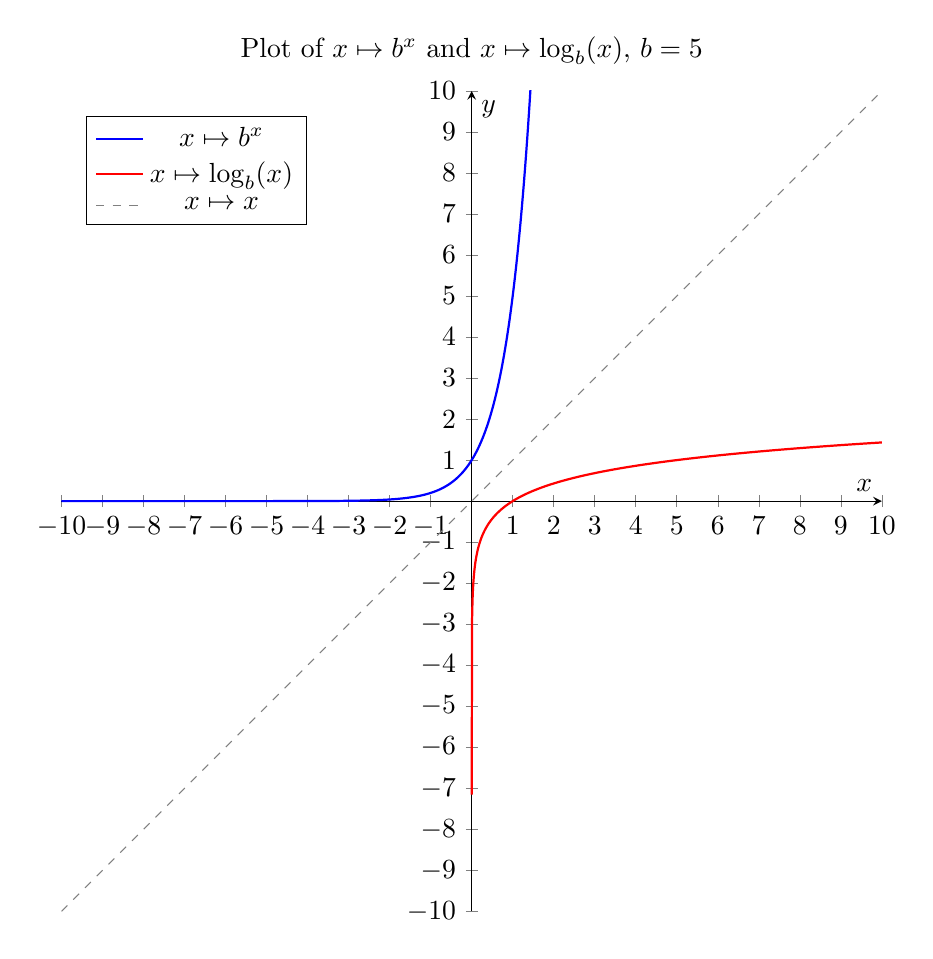
\begin{tikzpicture}
\begin{axis}[
    axis lines = center,
    xlabel = {$x$},
    ylabel = {$y$},
    xmin = -10, xmax = 10,
    ymin = -10, ymax = 10,
    xtick = {-10,-9,...,10},
    ytick = {-10,-9,...,10},
    width = 12cm,
    height = 12cm,
    samples = 1000,
    legend pos = north west,
    title = {Plot of $x \mapsto b^x$ and $x \mapsto \log_b(x)$, $b = 5$},
]
\addplot[blue, thick, domain=-10:2.5] {5^x};
\addplot[red, thick, domain=0.00001:10] {ln(x)/ln(5)};
\addplot[gray, dashed, domain=-10:10] {x};
\legend{$x \mapsto b^x$, $x \mapsto \log_b(x)$, $x \mapsto x$}
\end{axis}
\end{tikzpicture}
\end{center}

The graph helps us see some important characteristics of logarithms:

\begin{itemize}
    \item For all $b > 0$, since the domain and range of $x \mapsto b^x$ are $(-\infty, \infty)$ and $(0, \infty)$, respectivey, the domain and range of $\log_b$ are $(0, \infty)$ and $(-\infty, \infty)$, respectively. 
    \item Since $b^0 = 1$, then $\log_b(1) = 0$ for all $b > 0$.
    \item Since $\lim_{x \rightarrow -\infty} = 0$, then $\lim_{x \rightarrow 0} \log_b(x) = -\infty$ for all $b > 0$.
\end{itemize}

We also have the algebraic relationship

\begin{align*}
    \log_b(b^x) = x = b^{\log_b(x)} \text{ for all $x > 0$ and $b > 0$}.
\end{align*}

This is simply a restatement of the fact $f_b^{-1}(f_b(x)) = x = f_b(f_b^{-1}(x))$ for all $x > 0$ and $b > 0$.

\subsubsection*{The first property of logarithms}

Since exponential functions and logarithms are inverses, then for every property of exponents there must be a corresponding property of logarithms. The first of these properties is as follows:

\begin{itemize}
    \item $\log_b(xy) = \log_b(x) + \log_b(y)$ for all $x, y > 0$ and $b > 0$
\end{itemize}

Here, we give an intuitive explanation- not quite a proof- for this property. Later, we will fully nail it down with a proof.

Let $b, C > 0$. Consider that if $f_C(x) = C b^x$, then $f_C^{-1}(x) = \log_b(\frac{x}{C})$. We can interpret $f_C$ as describing the exponential growth of some quantity, where the initial amount of that quantity is $C$ (since $f(0) = Cb^0 = C$). Since $f_C^{-1}$ is the inverse to $f$, we can interpret $f_C^{-1}(x)$ as describing the amount of time needed to produce $x$ amount of the quantity, assuming that the initial amount of the quantity was $C$ and that the quantity grows by a multiplicative factor of $b$ for every $1$ unit of time:

\begin{align*}
    \text{time to grow from $C$ to $x$} = \log_b\left(\frac{x}{C}\right).
\end{align*}
                
Then, we can ask: how much time would it take to produce an amount $xy$ of the quantity, given that we are starting with an initial amount $1$? There are two ways to grow to $xy$. We can either have the quantity grow from $1$ to $x$ and then from $x$ to $xy$, or just have the quantity grow from $1$ to $xy$:

\begin{align*}
    &(\text{time to grow from $1$ to $x$}) + (\text{time to grow from $x$ to $xy$}) =     (\text{time to grow from $1$ to $xy$}) \\
    &\log_b\left(\frac{x}{1}\right) + \log_b\left(\frac{xy}{x}\right) = \log_b\left(\frac{xy}{1}\right) \\
    &\log_b(x) + \log_b(y) = \log_b(xy)
\end{align*}

Thus

\begin{align*}
    \log_b(xy) = \log_b(x) + \log_b(y) \text{ for all $x, y > 0$ and $b > 0$}.
\end{align*}

% There's additional insight to be had here. Since we treat the denominator $C$ as the initial amount, then we see that the time it takes to grow the quantity by a multiplicative factor of $u$ is always the same: this is formally expressed by the fact that $f^{-1}_{u_n}(u_{n + 1}) = \log_b(\frac{u^{n + 1}}{C u^n}) = \log_b(\frac{u}{C})$. We see that, specifically, the amount of time to grow the quantity by the multiplicative factor of $u$ is $\log_b(\frac{u}{C})$, which is the amount of time it takes to grow the quantity from $C$ to $u$.

\subsubsection*{Properties of logarithms}

Having explained the first property of logarithms, we are now ready to understand all of the properties. Since there were three properties of exponential functions, there are three properties of logarithms:

\begin{enumerate}
    \item $\log_b(xy) = \log_b(x) + \log_b(y)$ for all $x, y > 0$ and $b > 0$.
    \item $\log_b(x^y) = y\log_b(x)$ for all $x, y > 0$ and $b > 0$.
    \item When $b > 0$, the function $x \mapsto \log_b(x)$ is continuous, one-to-one, and maps to all real numbers.
\end{enumerate}

Here are the proofs:

\begin{enumerate}
    \item[1.] Though we prefer to keep in mind the previously given intuitive argument in mind as the primary reason for why this property of logarithms is true, we should still give a formal proof, just to be extra sure we didn't miss anything.
    
    (Proof). Start by considering the first property of exponential functions: $b^x b^y = b^{x + y} \text{ for all $x, y$}$. Now, impose the constraint $b > 0$ so that we can take the logarithm of each side of this equation. Doing so, we obtain $\log_b(b^x b^y) = x + y$. Then, setting $u = b^x \iff x = \log_b(u)$ and $v = b^y \iff y = \log_b(v)$, and noting that since $b > 0$ we must have $u, v > 0$, we obtain another equivalent equation: $\log_b(uv) = \log_b(u) + \log_b(v)$ for all $u, v > 0$ and $b > 0$. After renaming $u$ to $x$ and $v$ to $y$, we have $\log_b(xy) = \log_b(x) + \log_b(y)$ for all $x, y > 0$ and $b > 0$, as claimed.

    \item[3.] The third property is just straightforwardly a rephrasing of the corresponding property for exponential functions.
    
    \item[2.] While we can give a formal proof for the second property that's very similar to the one for the first property, we choose to give an alternative proof, which shows that- because logarithms are continuous- the second property is a natural consequence of the first. Since the first property ``makes sense'', the second, when viewed as a mere consequence of the first, should too.
    
    (Proof). Notice that for nonnegative integer values of $y$, the second property is an immediate consequence of the first property. What about for negative integer values of $y$? Let's consider $y = -1$. Since $\log_b(\frac{1}{x}) = -\log_b(x) \iff \frac{1}{x} = b^{-\log_b(x)} \iff \frac{1}{x} = (b^{\log_b(x)})^{-1} = x^{-1} \iff \frac{1}{x} = \frac{1}{x}$, the second property holds for $y = -1$. From here the first property can be applied again to prove the second property for all negative integer values of $y$, and thus all integer values of $y$. And, from here, it is simple enough to generalize the second property to all rational $y$. Once we know the second property is true for all rational $y$, the continuity of $\log_b$ when $b > 0$ forces it to be true for all real numbers $y$.
\end{enumerate}


\subsubsection*{Why ``logarithm''?}

You may be curious why the inverse of $x \mapsto b^x$ is called the ``logarithm''. It's quite a strange name.

The reason is that logarithms were first discovered in 1614, far before computers automated away the doing of arithmetic. Mathematicians needed a computational aid to help them multiply large numbers. The logarithm, having the property $\log_b(xy) = \log_b(x) + \log_b(y)$, and thus being able to convert the multiplication of many-digit numbers into addition of many-digit numbers, was the ideal tool for this. Mathematicians were therefore in the habit of thinking about the reorganized set of positive numbers that is obtained by applying a logarithm to every ``original'' positive number.

If we apply $\log_b$ for some $b > 0$ to all of the positive numbers, then numbers which were multiplicative factor apart in the ``original'' organization are now an additive difference apart in the ``new'' organization. That is, constant ratios between numbers in the ``original'' organization correspond to constant differences between numbers in the ``original'' organization:

\begin{align*}
    \frac{x}{y} = c \iff \log_b(x) - \log_b(y) = c.
\end{align*}

When a number was thought of as living in this ``new'' organization, it was called a  \textit{logarithm}, which means ``ratio-number'' in Greek, to allude to this property.

\subsubsection*{Logarithms, historically}

We now quickly give an idea of how mathematicians used logarithms to multiply large numbers. Specifically, mathematicians had tables of precomputed logarithm values, like this:

\begin{table}[h]
\centering
\begin{tabular}{|c|c|}
    \hline
    \textbf{$x$} & \textbf{$\log_{10}(x)$} \\
    \hline
        1.0000 & 0.0000 \\
    \hline
        1.0005 & 0.0022 \\
    \hline
        \vdots & \vdots \\
    \hline
        7.0065 & 0.8455 \\
    \hline
    \vdots & \vdots \\
    \hline
        1234 & 3.0913 \\
    \hline
    \vdots & \vdots \\
    \hline
        5678 & 3.7542 \\
    \hline
\end{tabular}
\label{tab:sample}
\end{table}

(In reality, logarithm tables were not just simple two-column tables; reading logarithm values from the actual tables involved some additional computation. We omit those details. Our two-column table is sufficient for presenting the core ideas.)

To multiply two many-digit numbers, like 1234 and 5678, one would first use logarithms to convert multiplication into addition. For readability, define $\text{exp}_{10}(x) := 10^x$. We have

\begin{align*}
    1234 \cdot 5678 &= \text{exp}_{10}(\log_{10}(1234 \cdot 5678)) = \text{exp}_{10}(\log_{10}(1234) + \log_{10}(5678)).
\end{align*}

Now we use the table to approximate the logarithms in the sum. From the table, we can see $\log_{10}(1234) \approx 3.0913$ and $\log_{10}(5678) \approx 3.7542$, so

\begin{align*}
    \text{exp}_{10}(\log_{10}(1234) + \log_{10}(5678)) \approx \text{exp}_{10}(3.0913 + 3.7542) = \text{exp}_{10}(6.8455) = 10^{6.8455}.
\end{align*}

In all, we have

\begin{align*}
    1234 \cdot 5678 \approx 10^{6.8455}.
\end{align*}

To complete the computation, we express $10^{6.8455}$ as $10^{6 + 0.8455} = 10^{0.8455} \cdot 10^6$. We leave the whole number power of $10$, which is $10^6$ in this case, alone, and consider it to be fully simplified. The fractional power of $10$, which is $10^{0.8455}$ in this case, is what we focus on. To compute $10^{0.8455}$, we just take advantage of the fact that $\log_{10}(10^{0.8455}) = 0.8455$, and look in the output column of the logarithm table for the exponent $0.8455$; the value of $10^{.08455}$ will be in the input column of the same row. Reading from the table in this way, we have

\begin{align*}
    1234 \cdot 5678 \approx 10^{6.8455} = 10^{0.8455} \cdot 10^6 \approx 7.0065 \cdot 10^6.
\end{align*}

This computation only differs from the exact answer $1234 \cdot 5678 = 7.006652 \cdot 10^6$ by an amount less than $.0001$, so we can see this method is pretty accurate.

\subsection*{Changes of base}

\subsubsection*{Change of base for exponential functions}

The \textit{change of base for exponential functions} is the fact that, for any real numbers $a, b$ with $b > 0$,

\begin{align*}
    a^x = b^{\log_b(a^x)} = b^{\log_b(a) x}.
\end{align*}

That is, for any $a, b$ with $b > 0$, we have

\begin{align*}
    a^x = b^{dx}, \text{ where $d = \log_b(a)$}.
\end{align*}

So, it doesn't really matter what base one uses in an exponential function, since any base can be ``converted'' to another base with the above formula.

\subsubsection*{Change of base for logarithms}

We can derive a way to change the base of a logarithm from our knowledge of the change of base for exponential functions. Start with the change of base of exponential functions, and take $\log_b$ of both sides to obtain $\log_b(a^x) = dx$. Let $y = a^x$ to obtain that ${\log_b(y) = d\log_a(y)}$, where $d = \log_b(a)$. Swapping $a$ and $b$ and replacing $y$ with $x$, we have the \textit{change of base for logarithms}:

\begin{align*}
    \log_a(x) = d\log_b(x), \text{ where $d = \log_a(b)$}.
\end{align*}

The change of base for logarithms is often stated as

\begin{align*}
    \log_b(x) = \frac{\log_a(x)}{\log_a(b)}.
\end{align*}

Note that the change of base for logarithms implies that when $x > 0$,

\begin{align*}
    \log_x(b) = \frac{\log_a(b)}{\log_a(x)} = \frac{1}{\log_b(x)}.
\end{align*}

\subsection*{Derivatives of exponential functions}

Given a real number $b > 0$, let's take the derivative of $b^x$ with respect to $x$.

\begin{align*}
    \frac{d}{dx} b^x = \lim_{h \rightarrow 0} \frac{b^{x + h} - b^x}{h}
    = \lim_{h \rightarrow 0} \frac{b^x (b^h - 1)}{h}
    = \Big( \lim_{h \rightarrow 0} \frac{b^h - 1}{h} \Big) b^x
\end{align*}

Notice that the limit in this last expression can be rewritten:

\begin{align*}
    \lim_{h \rightarrow 0} \frac{b^h - 1}{h} = \lim_{h \rightarrow 0} \frac{b^{0 + h} - b^0}{h} = \Big( \frac{d}{dx} b^x \Big)\Big|_0.
\end{align*}

Thus, the derivative of $b^x$ with respect to $x$ is

\begin{align*}
   \frac{d}{dx} b^x = \Big( \frac{d}{dx} b^x \Big)\Big|_0 b^x = f(b) b^x, \text{ where $f(b) = \Big( \frac{d}{dx} b^x \Big)\Big|_0$}.
\end{align*}

That is, the derivative of $b^x$ with respect to $x$ is the evaluation of some function at $b$, times $b^x$. In order to obtain a more useful expression for $\frac{d}{dx} b^x$, we must evaluate the expression $f(b)$. A natural way to do so is to first consider the $b$ for which\footnote{Does such a $b$ even exist? Does $\Big( \frac{d}{dx} b^x \Big)\Big|_0 = \lim_{h \rightarrow 0} \frac{b^h - 1}{h}$ even converge for all $b$? The answer to both questions is yes, but showing so is quite technical.} we have $f(b) = 1$.

For the sake of having concrete notation, we will \textit{define} $e$ to be the real number such that $f(e) = 1$. Then

\begin{align*}
    \frac{d}{dx} e^x = f(e) e^x = 1 \cdot e^x = e^x.
\end{align*}

Now, we use change of base for exponential functions in order to determine $\frac{d}{dx} b^x$ by making use of the fact that we know the derivative of $e^x$. We have

\begin{align*}
    \frac{d}{dx} b^x = \frac{d}{dx} e^{\log_e(b^x)} = \frac{d}{dx} e^{\log_e(b) x} = \log_e(b) e^{\log_e(b^x)} = \log_e(b) b^x.
\end{align*}

In all,

\begin{align*}
    \frac{d}{dx} b^x = \log_e(b) b^x.
\end{align*}

In some sense, $e$ is the ``most natural exponent'' because it is the one for which $\frac{d}{dx} e^x = 1 \cdot e^x$. For this reason, the logarithm of base $e$ is called the \textit{natural logarithm}, and is denoted by $\ln$ (for ``logarithmus naturali''). Formally, we define $\ln := \log_e$. So the above is restated as

\begin{align*}
    \boxed
    {
        \frac{d}{dx} b^x = \ln(b) b^x
    }
\end{align*}

\subsubsection*{Alternate expression for $e^x$}

We now make a series of observations that lead us to an alternate expression for $e^x$. To start, recall that we \textit{defined} $e$ to be such that $\Big( \frac{d}{dx} e^x \Big)\Big|_0 = 1$. Also recall that, for any function $f$, the derivative of the inverse function $f^{-1}$ is given by:

\begin{align*}
    \frac{df^{-1}(y)}{dy} = \frac{1}{\frac{df(f^{-1}(y))}{df^{-1}(y)}} \text{for all $y$ such that $\frac{df(f^{-1}(y))}{df^{-1}(y)} \neq 0$}.
\end{align*}

We can substitute $f(x) = e^x$ and $y = 1$ into the above to obtain

\begin{align*}
    \frac{d\ln(1)}{d1} = \frac{1}{\frac{e^0}{d0}},
\end{align*}

which is more nicely written as

\begin{align*}
    \Big( \frac{d}{dy} \ln(y) \Big)\Big|_1 = \frac{1}{\frac{d}{dx}(e^x)|_0}.
\end{align*}

Since $\frac{d}{dx}(e^x)|_0 = e^x|_0 = e^0 = 1$, we have

\begin{align*}
    \Big(\frac{d}{dy} \ln(y)\Big)\Big|_1 = 1.
\end{align*}

Computing the derivative of $\ln(x)$ at $x = 1$ explicitly, we have

\begin{align*}
    \lim_{h \rightarrow 0} \frac{\ln(1 + h) - \ln(1)}{h} = \lim_{h \rightarrow 0} \frac{\ln(1 + h)}{h} = \lim_{h \rightarrow 0} \ln((h + 1)^\frac{1}{h}) = 1.
\end{align*}

Interestingly enough, a not yet encountered expression for $e$ jumps out at us from this above equation. Apply the function $x \mapsto e^x$ to both sides of the above (using continuity to bring the application of $x \mapsto e^x$ inside the limit) to obtain

\begin{align*}
    \lim_{h \rightarrow 0} (h + 1)^{\frac{1}{h}} = e,
\end{align*}

and then substitute $k := \frac{1}{h}$ to obtain

\begin{align*}
   \lim_{k \rightarrow \infty} \Big( \frac{1}{k} + 1 \Big)^k = e.
\end{align*}

Substituting $n$ in for $k$, we see that we have shown

\begin{align*}
    e &= \lim_{n \rightarrow \infty} \Big(1 + \frac{1}{n} \Big)^n.
\end{align*}

We now use this new expression for $e$ to determine a new expression for $e^x$. Applying the function $x \mapsto e^x$ to both sides of the above, we see that for all $x$,

\begin{align*}
    e^x = \Big( \lim_{n \rightarrow \infty} \Big(1 + \frac{1}{n} \Big)^n \Big)^x = \lim_{n \rightarrow \infty} \Big(1 + \frac{1}{n}\Big)^{nx}.
\end{align*}

Substitute $p := nx$ to obtain

\begin{align*}
    e^x = \lim_{p \rightarrow \infty} \Big( 1 + \frac{x}{p} \Big)^p.
\end{align*}

Overall, we have shown

\begin{empheq}[box = \fbox]{align*}
    e &= \lim_{n \rightarrow \infty} \Big(1 + \frac{1}{n} \Big)^n \\
    e^x &= \lim_{n \rightarrow \infty} \Big(1 + \frac{x}{n} \Big)^n
\end{empheq}

\subsubsection*{$e$ and compound interest}

Calculus textbooks are overly fond of discussing how to interpret the fact that $e = \lim_{n \rightarrow \infty} \Big(1 + \frac{1}{n} \Big)^n$ in the setting of interest rates, so I include the below for completeness.
    
The argument of the limit, $(1 + \frac{1}{n})^n$, can be interpreted as the factor by which an initial quantity grows when the growth of the quantity occurs in $n$ stages and where the quantity grows by a factor of $1 + \frac{1}{n}$ in each stage. For example, if you put $\$100$ in the bank with a yearly interest rate of $\frac{1}{5} = 20\%$, and let this money sit in the bank for $5$ years, then your $\$100$ would have grown by a factor of $(1 + \frac{1}{5})^5 = (120 \%)^5 = 2.48832 = 248.832\%$ at the end of the $5$ years. So, you would have $\$100 \cdot 2.48832 = \$248.832$ at the end of the $5$ years.

We say that the money \textit{compounds} whenever it grows as a result of applying the interest rate. In the above scenario, the money is compounded $n = 5$ times, once at the end of each year. Taking the limit as $n \rightarrow \infty$ represents using a very small interest rate (an interest rate of $\frac{1}{n}$) infinitely often. Thus, $e$ can be interpreted as the factor by which quantities grow when subject to so-called \textit{continuously compounded} interest.

\subsubsection*{Common pedagogical problems with $e$, $e^x$ and $\ln(x)$}

You should be warned that the usual ways to present $e$, $e^x$ and $\ln(x)$ are all incredibly problematic. In fact, the unproblematic derivation and explanation of $e$, $e^x$ and $\ln(x)$ presented here is so uncommon that I have never read of it in another math textbook, and have only seen it discussed in an online blog by Paramanand Singh.

The problem with these usual ways is that every one of them starts by assuming the truth of one of our ``end results'' (such as $e = \lim_{n \rightarrow \infty} \Big(1 + \frac{1}{n} \Big)^n$ or $e^x = \lim_{n \rightarrow \infty} \Big(1 + \frac{x}{n} \Big)^n$, or even facts we haven't learned of yet, like ``$e = \sum_{n = 0}^\infty \frac{1}{n!}$'', ``$e^x = \sum_{n = 0}^\infty \frac{x^n}{n!}$'', and ``$\ln(x) = \int_1^x \frac{1}{x} dx$'') and then uses said ``end result'' as a starting point from which to establish the properties of $e$, $e^x$ and $\ln(x)$. This can technically be done without any formal logical error- but it is unintuitive and unnatural. Who could reasonably come up with the idea to use one of these ``end results'' as a starting point without doing a ridiculous amount of prior investigation? Well-explained math is math that feels at least somewhat plausible to discover, and starting with one of the mentioned ``end results'' is not of this spirit.

\subsection*{Derivatives of logarithms}

We already know how to take the derivative of an exponential function. Since the logarithm $\log_b$, $b > 0$, is the inverse of the exponential function $f_b$ defined by $f_b(x) = b^x$, we can determine the derivative of $\log_b$ from the general formula for derivatives of inverse functions. Applying that formula to $f_b^{-1} = \log_b$, we have

\begin{align*}
    \frac{df_b^{-1}(y)}{dy} = \frac{1}{\frac{df_b(f_b^{-1}(y))}{df_b^{-1}(y)}} \text{for all $y$ such that $\frac{df_b(f_b^{-1}(y))}{df_b^{-1}(y)} \neq 0$}.
\end{align*}

This is equivalent to

\begin{align*}
    \frac{d\log_b(y)}{dy} = \frac{1}{\frac{d}{d\log_b(y)}f_b(\log_b(y))} \text{ for all $y$ such that $\frac{d}{d\log_b(y)}f_b(\log_b(y)) \neq 0$}.
\end{align*}

Since $\frac{d}{dx}f_b(x) = \frac{d}{dx} b^x = \ln(b) b^x$, we have $\frac{d}{d\log_b(y)}f_b(\log_b(y)) = \ln(b) b^{\log_b(y)} = \ln(b) y$. Thus the above is equivalent to

\begin{align*}
    \frac{d\log_b(y)}{dy} = \frac{1}{\ln(b) y} \text{ for all $y \neq 0$}.
\end{align*}

Renaming $y$ to $x$, we have

\begin{align*}
    \boxed
    {
        \frac{d\log_b(x)}{dx} = \frac{1}{\ln(b) x} \text{ for all $x \neq 0$}
    }
\end{align*}

In particular, for $\ln = \log_e$, we have

\begin{align*}
    \boxed
    {
        \frac{d\log_b(x)}{dx} = \frac{1}{x} \text{ for all $x \neq 0$}
    }
\end{align*}

A nice sanity check is that when we use the change of base for logarithms to derive the derivative of $\log_b$ from the derivative $\ln$, the result we get agrees with what we already derived:

\begin{align*}
    \frac{d}{dx}\log_b(x) = \frac{d}{dx}\left( \frac{\ln(x)}{\ln(b)} \right) = \frac{1}{\ln(b)} \frac{d}{dx} \ln(x) = \frac{1}{\ln(b) x}.
\end{align*}

This can be a useful way to remember the derivative of $\log_b$ if you forget it but still remember the simpler derivative of $\ln$.

\section*{Analytical geometry}

\begin{itemize}
    \item Increasingness, decreasingness, local/global extrema
    \begin{itemize}
        \item Extreme value theorem: if an extremum of $f$ occurs at $x$, then $\frac{df}{dx}\Big|_x = 0$.
        \begin{itemize}
            \item The converse of extreme value theorem is not true: it is not necessarily true that if $\frac{df}{dx}\Big|_x = 0$, then $x$ is an extreme value of $f$.
        \end{itemize}
    \end{itemize}
    \item Concavity, inflection points
    \item Horizontal and vertical asymptotes
\end{itemize}

\section*{Misc.}

\begin{itemize}
    \item Mean value theorem
    \begin{itemize}
        \item Isn't ``misc'' if you're proving calculus, but is ``misc'' if you're using calculus.
    \end{itemize}
    \item L'Hopital's rule
\end{itemize}

\newpage

\part*{Integral calculus}

\section*{Riemann sums and definite integrals}

\subsection*{Riemann sums}

Given the derivative $f'$ of some function $f$, we can approximate the change in $f$ from $x = a$ to $x = b$, which is $f(b) - f(a)$, as follows. First, we break up the interval $[a, b]$ into many intervals:

\begin{align*}
    [x_1, x_2] = [a, x_2], [x_2, x_3], ..., [x_{n - 1}, x_n] = [x_{n - 1}, b], \text{ where $x_{i + 1} > x_i$}.
\end{align*}

Next, we approximate $f'$ as a piecewise function that is constant on each piece. For a particular ``piece'' $[x_i, x_{i + 1}]$, we pick one of the values that $f'$ takes on within this interval, and then define our piecewise approximation to be equal to this value when evaluated on any input inside the same interval.

Lastly, we apply the formula $(\text{change in output}) = (\text{rate of change}) \cdot (\text{change in input})$, which is true for constant rates of change, on each piece, and sum up the changes in output of all the pieces to obtain an approximation of the total change in $f$ from $x = a$ to $x = b$. The approximation gets better as we use more pieces. 

Symbolically, all the previous steps combine to tell us that the change in $f$ from $x = a$ to $x = b$ is approximately:
 
\begin{align*}
    f(b) - f(a) \approx \sum_{i = 1}^n \frac{df}{dx}\Big|_{x = p_i} (\Delta x)_i, \text{ where $(\Delta x)_i = x_{i + 1} - x_i$},
\end{align*}

and where we choose $p_i$ in one of the following ways:

\begin{align*}
 p_i &= x_i \text{ for a \textit{left Riemann sum}} \\
 p_i &= x_i + \frac{(\Delta x_i)}{2} \text{ for a \textit{midpoint Riemann sum}} \\
 p_i &= x_{i + 1} \text{ for a \textit{right Riemann sum}}.
\end{align*}

The choice of $p_i$ determines which value our piecewise approximation takes on in each piece; for example, if a left Riemann sum is chosen, then the piecewise approximation takes on the ``leftmost'' value of $f$ within that piece.

We have used the words ``Riemann sum'' in the above definition of $p_i$, but not explained what ``Riemann sum'' means. What is a Riemann sum? A \textit{Riemann sum of a function $g$ from $a$ to $b$} is a sum of the form

\begin{align*}
    \sum_{i = 1}^n g(p_i) (\Delta x)_i, \text{ where $(\Delta x)_i = x_{i + 1} - x_i$},
\end{align*}

where the intervals $[x_i, x_{i + 1}]$ are chosen in the same way as above (in particular, we must have $x_1 = a$ and $x_n = b$), and where the $p_i$ are chosen in one of the ways described above.

So, the above sum involving $\frac{df}{dx}\Big|_{x = p_i}$ is a Riemann sum of $x \mapsto \frac{df}{dx}\Big|_x = \frac{df(x)}{dx}$ from $a$ to $b$; it is a Riemann sum of $f'$ from $a$ to $b$.

\subsubsection*{Riemann sums and area}

If one has a function $g$ and draws a graph of $g$ vs. $x$, they can notice that $g(p_i) (\Delta x)_i$ is the width of the rectangle with height $g(p_i)$ and width $(\Delta x)_i$. So, a Riemann sum of $g$ from $a$ to $b$ approximates the area under the graph of $g$ that is above the $y$-axis and between the vertical lines $x = a$ and $x = b$.

\subsection*{The definite integral}

We define the \textit{definite integral from $a$ to $b$} of a function $g$ to be the following limit of a Riemann sum:

\begin{align*}
    \int_a^b g(x) dx := \lim_{\max((\Delta x)_i) \rightarrow 0} \sum_{i = 1}^n g(p_i) (\Delta x)_i, \text{ where $p_i$ is any of the above}.
\end{align*}

In the limit, the maximum input interval $\max((\Delta x)_i)$ approaches $0$, so all other input intervals are forced to approach $0$ as well. Thus, the above limit corresponds to approximating the change in $g$ when $g$ is approximated as a piecewise function of ``infinitely many'' pieces.

Since a Riemann sum of $x \mapsto \frac{df(x)}{dx}$ from $a$ to $b$ approximates the change in $f$ over this input interval,

\begin{align*}
     f(b) - f(a) \approx \sum_{i = 1}^n \frac{df}{dx}\Big|_{x = p_i} (\Delta x)_i,
\end{align*}

it stands to reason that the definite integral of $x \mapsto \frac{df(x)}{dx}$ from $a$ to $b$, being an ``infinitely accurate Riemann sum'', will be equal to this change:

\begin{align*}
    f(b) - f(a) = \int_a^b \frac{df}{dx}\Big|_x dx = \int_a^b \frac{df(x)}{dx} dx.
\end{align*}

This is indeed true.

\subsubsection*{The definite integral and area}

In the previous section, we noted that ``a Riemann sum of $g$ from $a$ to $b$ approximates the area under the graph of $g$ that is above the $y$-axis and between the vertical lines $x = a$ and $x = b$''. Since an integral is intuitively an ``infinitely accurate Riemann sum'', the exact area under the graph of $g$ from $a$ to $b$ is $\int_a^b g(x) dx$.

\section*{Antiderivatives and the fundamental theorem of calculus}

Our investigation of Riemann sums and definite integrals showed that we can compute the change in a function $f$ over an input interval $x = a$ to $x = b$ as

\begin{align*}
    f(b) - f(a) = \int_a^b \frac{df(x)}{dx} dx.
\end{align*}

Since any continuous function is the derivative of some other continuous function, we can rewrite the above by interpreting $x \mapsto \frac{df(x)}{dx}$ to be an arbitrary continuous function $g$:

\begin{align*}
    ? = \int_a^b g(x) dx
\end{align*}

We used a question mark in the above because it is somewhat unclear how to convert the previous left side of the equation, $f(b) - f(a)$, into an expression that involves $g$ rather than $f$.

In order to figure out what $?$ is, notice that in the equation $f(b) - f(a) = \int_a^b \frac{df(x)}{dx} dx$, the function on the right side, $x \mapsto \frac{df(x)}{dx}$, is the derivative of the function on the left side, $f$. So it stands to reason that in the above equation, the function $g$ on the right side is the derivative of whatever function is involved in the left side. Therefore, we will guess that

\begin{align*}
    G(b) - G(a) = \int_a^b g(x) dx, \text{ where for all $x$ we have $\frac{dG(x)}{dx} = g(x)$}.
\end{align*}

In order to prove that this guess is correct, we must think more about the function $G$.

In general, any function $H$ that satisfies $H' = g$ is said to be an \textit{antiderivative of $g$}. (Thus, the $G$ above is an antiderivative of $g$). Observe that there are many antiderivatives of any function, since, if $H$ is an antiderivative of $g$ and $c$ is a constant, then $H + c$ must be an antiderivative of $g$ as well\footnote{For all $x$, we have $\frac{d}{dx}(H(x) + c) = \frac{dH(x)}{dx} + 0 = \frac{dH(x)}{dx} = g(x)$.}. 

In fact, one can show that \textit{any} two antiderivatives of a function must differ by a constant\footnote{Suppose $F$ and $G$ are both antiderivatives of $g$. Then $F' = G'$, so $F' - G' = 0$. Using the linearity of the derivative, we have $(F - G)' = 0$. It follows from the mean value theorem that if a function's derivative is zero for all inputs, then the function must be a constant function. Applying this fact to the function $F - G$, we see that $F - G$ must be a constant function. That is, $F$ and $G$ differ by a constant.}. This is very important- it means that if you've found one antiderivative of a function, you've really found all its antiderivatives: the collection of all antiderivatives is equal to the collection of functions obtained by adding constants to the one antiderivative you found.

Now, we can justify our above guess; we can justify why the old left side $f(b) - f(a)$ is equal to the new left side $G(b) - G(a)$. The justification is as follows. Since $f$ and $G$ are antiderivatives of $f' = g$, they differ by a constant: for each $x$, we have $f(x) = g(x) + d$ for some constant $d$. This implies that $f(b) - f(a) = (G(b) + d) - (G(a) + d)) = G(b) - G(a)$, as we claimed.

We now restate the equation above, with the only change being that we use the letters $f$ and $F$ instead of $g$ and $G$. This equation is called the \textit{the second part of the fundamental theorem of calculus}. We will abbreviate it as \textit{FTC 2}.

\begin{align*}
    \text{If $F$ is an antiderivative of $f$ then $\int_a^b f(x) dx = F(b) - F(a)$.}
\end{align*}

If $x$ is substituted for $b$, FTC 2 can be written as

\begin{align*}
    \text{If $F$ is an antiderivative of $f$ then $F(x) = \int_a^x f(x) dx + F(a)$ for all $x$}.
\end{align*}

This shows that any antiderivative can be written as a definite integral plus a constant. For this reason, the taking of an antiderivative is notated with an integral symbol without limits of integration:

\begin{align*}
    \text{``$F(x) = \int f(x) dx$ for all $x$'' means ``$F$ is an antiderivative of $f$''}.
\end{align*}

Such integrals without limits are called \textit{indefinite}. With this new notation, FTC 2 can be written as

\begin{align*}
    \text{If $F(x) = \int f(x) dx$ for all $x$ then $\int_a^b f(x) dx = F(b) - F(a)$}.
\end{align*}

\textit{The first part of the fundamental theorem of calculus} follows as a logical consequence of the second part. From above, we have

\begin{align*}
    \text{If $F$ is an antiderivative of $f$ then $F(x) = \int_a^x f(x) dx + F(a)$ for all $x$}.
\end{align*}

Take the derivative of both sides of the equation with respect to $x$ to obtain \textit{the first part of the fundamental theorem of calculus}, which we abbreviate as \textit{FTC 1}:

\begin{align*}
    f(x) = \frac{d}{dx} \int_a^x f(x).
\end{align*}

We restate FTC 2 and FTC 1 for convenience:

\begin{empheq}[box = \fbox]{align*}
    \text{If $F(x) = \int f(x) dx$ for all $x$ then $\int_a^b f(x) dx$} &= F(b) - F(a), \\
    \frac{d}{dx} \int_a^x f(x) &= f(x)
\end{empheq}

\vspace{.5cm}

FTC 2 and FTC 1 formalize the sense in which antiderivatives and definite integrals are related. FTC 2 says that definite integrals can be computed by evaluating antiderivatives. FTC 1 says that the function $x \mapsto \int_a^x f(x) dx$, which involves a definite integral, is an antiderivative of $f$.

Note that the previous sentence implies:

\begin{align*}
    \boxed
    {
        \text{Every continuous function has an antiderivative.}
    }
\end{align*}

Contrastingly, recall that it is \textit{not} the case that every continuous function has a derivative.

\subsubsection*{Why FTC 2 before FTC 1?}

We've proved FTC 2 implies FTC 1. It's also possible to prove FTC 1 implies FTC 2. 

In my opinion, FTC 2 is more intuitive than FTC 1. FTC 1 says ``the rate of change of the `accumulation' of $f$ is equal to $f$ itself'', which seems a bit complicated for someone to intuit. FTC 2, which says that adding up many ``infinitesimal'' changes gives an overall change, seems to be a much easier discovery. Since FTC 1 is easily seen to follow from FTC 2, I think that treating FTC 2 as the fundamental principle and FTC 1 as a corollary is the way to go.

\subsection*{Integral notation}

Before we proceed further, we should define some conventions for notating integrals. So far, the only conventions we've established are that that the definite integral of a function $f$ from $a$ to $b$ is written as $\int_a^b f(x) dx$ and that the evaluation at $x$ of an antiderivative of a function $f$ is written as $\int f(x) dx$. 

We now lay out new conventions analogous to prime notation\footnote{The notations $\int f$, $\int_a^b f$, and $f'$ are analogous because they are concern functions, not functions evaluated on inputs.} for derivatives:

\begin{align*}
    \int f := \text{an antiderivative of $f$}, &\quad \int_a^b f := \text{the definite integral of $f$ from $a$ to $b$}.
\end{align*}

With these new conventions, we can restate the already established integral notation more clearly:

\begin{align*}
    \int f(x) dx := \Big(\int f\Big)\Big|_x, &\quad \int_a^b f(x) dx := \int_a^b f.
\end{align*}

We also define integral notation analogous to the Leibniz notation $\frac{df(g(x))}{dg(x)} := f'(g(x))$:

\begin{align*}
    \int f(g(x)) dg(x) := \Big(\int f\Big)\Big|_{g(x)}, \quad \int_a^b f(g(x)) dg(x) := \Big(\int_a^b f\Big)\Big|_{g(x)}.
\end{align*}

\vspace{.5cm}

Lastly, we define the vocabulary word \textit{integrand}. The integrand of an integral is just the argument of that integral. So, the integrand of $\int f$ is $f$ and the integrand of $\int f(x) dx$ is $f(x)$.

\section*{Integration formulas}

[Pull from introduction of next section to write intro to this section]

\subsection*{The power rule}

\subsection*{Linearity of the integral}

\subsection*{Integrals of trig functions}

\subsection*{Integrals of inverse functions}

\subsection*{Integrals via inverse trigonometry}

\subsection*{Integrals of exponential and logarithmic functions}

When $x > 0$, we have $\int \frac{1}{x} dx = \ln(x)$. We don't have $\int \frac{1}{x} dx = \ln(x)$ when $x < 0$ because $\ln(x)$ isn't even defined when $x < 0$.

To find an antiderivative for $x \mapsto \frac{1}{x}$ for all $x$, notice that $\ln(|x|)$ is defined for all $x$. Is $x \mapsto \ln(|x|)$ an antiderivative of $x \mapsto \frac{1}{x}$, though? We do a quick check, and find out it is:

\begin{align*}
    \frac{d}{dx} \ln(|x|) = 
    \frac{1}{|x|} \frac{d|x|}{dx} =
    \frac{1}{|x|} \frac{d}{dx}
    \Bigg(
    \begin{cases}
        x & x \geq 0 \\
        -x & x < 0
    \end{cases}
    \Bigg)
    =
    \frac{1}{|x|} 
    \Bigg(
    \begin{cases}
        1 & x \geq 0 \\
        -1 & x < 0
    \end{cases}
    \Bigg)
    = \frac{1}{x}.
\end{align*}

So in all, we have 

\begin{align*}
    \boxed
    {
        \int \frac{1}{x} dx = \ln(|x|)
    }
\end{align*}

People often write $\ln(|x|)$ as simply $\ln|x|$.

\subsection*{etc.}

$\int_a^b = -\int_b^a$

\section*{The inverse chain rule}
    
[change below text to introduce the idea of the ``inverse'' chain rule]
    
In this section, we derive several integration formulas. We often do so by starting with a differentiation formula, taking the antiderivative of both sides, and interpreting some derivative that appears in the resulting expression to be ``just a regular function''. Such interpretations are valid because FTC 1 tells us that every continuous function has an antiderivative. Because integral formulas make use of this interpretation in their derivations, they all require that certain derivatives are continuous; i.e., they all require that certain functions are ``continuously differentiable''. 

In spite of the above note about ``continuous differentibility'', I will not be a stickler about stating the conditions that must be satisfied for a fact about integrals to be applicable, just as was the case when deriving derivative formulas. I will make note of conditions when doing derivations, but will not restate them in final ``boxed'' formulas. Conditions for integral formulas are in general less self-evident than those for derivative formulas, but you can still determine good guesses as to what the conditions are by starting with the corresponding derivative formula and integrating both sides.

\subsection*{Change of variables theorem}

First, we will derive the fact for integrals that corresponds to the chain rule for derivatives. Recall that the chain rule can be stated as

\begin{align*}
    (g \circ f)' = (g' \circ f) \circ f'.
\end{align*}

Integrate both sides to obtain

\begin{align*}
    g \circ f = \int (g' \circ f) \circ f'.
\end{align*}

Now, we will think of $g'$ as being ``just a regular function''. To formalize this, substitute $h := g'$. This implies\footnote{We need to justify that $h$ has an antiderivative here. In order for this to be guaranteed, we actually needed to assume at the beginning that $g$ is \textit{continuously differentiable}, i.e., that $g'$ is continuous. This is a pretty technical detail, so we don't mention it outside this footnote.} $g = \int h$, and we have

\begin{align*}
    \Big( \int h \Big) \circ f = \int (h \circ f) f'.
\end{align*}

Now, substitute the letter $g$ in for the letter $h$, and ``flip'' the equation around to obtain our primary result.

\begin{align*}
    \int (g \circ f) f' = \Big(\int g \Big) \circ f.
\end{align*}

Using the integral notation analogous to Leibniz notation, the primary result can be restated as

\begin{empheq}[box = \fbox]{align*}
    \int g(f(x)) \frac{df(x)}{dx} dx = \int g(f(x)) df(x)
\end{empheq}

This theorem makes the idea of ``canceling differentials'' within integrals rigorous, since it appears as if the $dx$ in the ``denominator'' of the integrand on the left side is canceled by the $dx$ that is the placeholder of the left side's integrand\footnote{A quicker proof, which you might discover if you suspected the primary result to be true is as follows. First, notice that the chain rule implies $\Big( \Big( \int g \Big) \circ f \Big)' = (g \circ f)f'$. Then integrate both sides.}.

The theorem is often stated with the substitutions $g = f$ and $f = u$:

\begin{empheq}[box = \fbox]{align*}
    \int f(u(x)) \frac{du(x)}{dx} dx = \int f(u(x)) du(x)
\end{empheq}

\subsection*{Separation of variables}

One important application of the change of variables theorem is the solving of so-called \textit{separable differential equations}, which are equations of the form 

\begin{align*}
    \frac{df(x)}{dx} = f(x) g(f(x)) \text{ for all $x$}.
\end{align*}

(In general, a \textit{differential equation} is an equation that involves a function and one or more of its derivatives).

To solve the above equation, we will apply the change of variables theorem and ``cancel differentials''.

Rephrasing the original equation, we have

\begin{align*}
    \frac{1}{g(f(x))} \frac{df(x)}{dx} = f(x) \text{ for all $x$ such that $g(f(x)) \neq 0$}.
\end{align*}

Integrate both sides to obtain

\begin{align*}
    \int \frac{1}{g(f(x))} \frac{df(x)}{dx} dx = \int f(x) dx \text{ for all $x$ such that $g(f(x)) \neq 0$}.
\end{align*}
 
Now use the change of variables theorem to ``cancel the $dx$'s on the left side'':

\begin{empheq}[box = \fbox]{align*}
    &\text{The solution to } \frac{df(x)}{dx} = f(x) g(f(x)) \text{ for all $x$ is } \\
    &\int \frac{1}{g(f(x))} df(x) = \int f(x) dx \text{ for all $x$ such that $g(f(x)) \neq 0$}.
\end{empheq}

In practice, we (attempt to) solve the separable differential equation by explicitly computing the above integrals and then using algebra to solve the above equation for $f$.

\subsubsection*{Mnemonic for separation of variables}

The solution to the differential equation

\begin{align*}
    \frac{df(x)}{dx} = f(x) g(f(x)) \text{ for all $x$}
\end{align*}

can be remembered by the mnemonic of doing algebra to ``put the $f$'s and $df(x)$'s on one side and put the $x$'s and $dx$'s on the other side''. We divide both sides by $g(f(x))$ to get the $f$'s and $df(x)$'s on the left side, and then ``multiply both sides by $dx$'' to get the $x$'s on the right side: 

\begin{align*}
    \frac{df(x)}{g(f(x))} = f(x) dx \text{ for all $x$ such that $g(f(x)) \neq 0$}.
\end{align*}

Now we ``integrate both sides'' of the above mnemonic expression to obtain

\begin{align*}
    \int \frac{1}{g(f(x))} df(x) = \int f(x) dx \text{ for all $x$ such that $g(f(x)) \neq 0$},
\end{align*}

exactly as before.

\section*{More integration formulas}

\subsection*{Integration by parts}

\begin{itemize}
    \item Is the ``reverse product rule''.
    \item $(fg)' = f'g + g'f$. Integrate both sides to obtain $fg = \int (f'g + g'f) = \int f'g + \int g'f$. Now subtract one of the integrals on the right side to obtain either
    
    \begin{align*}
        \int f'g = fg - \int fg'
    \end{align*}
    
    or
    
    \begin{align*}
        \int fg' = fg - \int f'g.
    \end{align*}
    
    It doesn't matter which of the above equations you use, as swapping $f$ and $g$ in one of the equations yields the other. We will consider the second equation,
    
    \begin{align*}
        \int fg' = fg - \int f'g.
    \end{align*}
    
    Substitute $h = g'$, so $g = \int h$. Then
    
    \begin{align*}
        \int fh = fH - \int f'H, \text{ where } H = \int h.
    \end{align*}
    
    Rewriting the above with the letters $f, g$, and $G$, we have
    
    \begin{align*}
        \boxed
        {
            \int fg = fG - \int f'G, \text{ where } G = \int g
        }
    \end{align*}
    
    When using the above formula, pick $f$ to be a function whose derivative is computable, and pick $G$ to be a function whose integral is computable.
    
    [insert spaces in integrals]
    
    \item We now present the most popular way to state the integration by parts formula. Above, we showed that

    \begin{align*}
        \int f(x) g'(x) \spc dx = f(x) g(x) - \int g(x) f'(x) \spc dx \text{ for all $x$}
    \end{align*}

    If we use the mnemonics ``$df(x) = f'(x) dx$'' and ``$dg(x) = g'(x) dx$'', we can write this formula as:

    \begin{align*}
        &\int f(x) dg(x) = f(x) g(x) - \int g(x) df(x), \\
        &\text{ where ``$dg(x) = g'(x) dx$'' and ``$df(x) = f'(x) dx$''}
    \end{align*}

    Note that the meanings of $df(x)$ and $dg(x)$ in the above are \textit{not} the same as the meanings that make most sense\footnote{The definition $\int f(g(x)) dg(x) := (\int f)|_{g(x)}$, which was given earlier, is what makes most sense.} Additionally, it is more work to memorize the above formula and the associated meanings of $df(x)$ and $dg(x)$ than it is to derive the above boxed formula from the product rule. Therefore, \textit{please ignore this formula.} It is included only for completeness.

    Unfortunately, the above formula is most commonly written with $u := f$ and $v := g$, in the even more sloppy notation ``${\int u \spc dv = uv - \int v \spc du}$''.
\end{itemize}